\PassOptionsToPackage{unicode=true}{hyperref} % options for packages loaded elsewhere
\PassOptionsToPackage{hyphens}{url}
%
\documentclass[english,man]{apa6}
\usepackage{lmodern}
\usepackage{amssymb,amsmath}
\usepackage{ifxetex,ifluatex}
\usepackage{fixltx2e} % provides \textsubscript
\ifnum 0\ifxetex 1\fi\ifluatex 1\fi=0 % if pdftex
  \usepackage[T1]{fontenc}
  \usepackage[utf8]{inputenc}
  \usepackage{textcomp} % provides euro and other symbols
\else % if luatex or xelatex
  \usepackage{unicode-math}
  \defaultfontfeatures{Ligatures=TeX,Scale=MatchLowercase}
\fi
% use upquote if available, for straight quotes in verbatim environments
\IfFileExists{upquote.sty}{\usepackage{upquote}}{}
% use microtype if available
\IfFileExists{microtype.sty}{%
\usepackage[]{microtype}
\UseMicrotypeSet[protrusion]{basicmath} % disable protrusion for tt fonts
}{}
\IfFileExists{parskip.sty}{%
\usepackage{parskip}
}{% else
\setlength{\parindent}{0pt}
\setlength{\parskip}{6pt plus 2pt minus 1pt}
}
\usepackage{hyperref}
\hypersetup{
            pdftitle={Article processing charges, the geographic diversity of author communities, and barriers to publication for authors in the Global South},
            pdfauthor={Audrey C. Smith,1, Leandra Merz,1, Jesse Borden1, Chris K. Gulick1, Akhil R. Kshirsagar1, \& Emilio M. Bruna1},
            pdfkeywords={Open access, article processing charges, author diversity, geographic diversity, Global South, mirror journals, Open Access},
            pdfborder={0 0 0},
            breaklinks=true}
\urlstyle{same}  % don't use monospace font for urls
\usepackage{graphicx,grffile}
\makeatletter
\def\maxwidth{\ifdim\Gin@nat@width>\linewidth\linewidth\else\Gin@nat@width\fi}
\def\maxheight{\ifdim\Gin@nat@height>\textheight\textheight\else\Gin@nat@height\fi}
\makeatother
% Scale images if necessary, so that they will not overflow the page
% margins by default, and it is still possible to overwrite the defaults
% using explicit options in \includegraphics[width, height, ...]{}
\setkeys{Gin}{width=\maxwidth,height=\maxheight,keepaspectratio}
\setlength{\emergencystretch}{3em}  % prevent overfull lines
\providecommand{\tightlist}{%
  \setlength{\itemsep}{0pt}\setlength{\parskip}{0pt}}
\setcounter{secnumdepth}{5}

% set default figure placement to htbp
\makeatletter
\def\fps@figure{htbp}
\makeatother

% Manuscript styling
\usepackage{upgreek}
\captionsetup{font=singlespacing,justification=justified}

% Table formatting
\usepackage{longtable}
\usepackage{lscape}
% \usepackage[counterclockwise]{rotating}   % Landscape page setup for large tables
\usepackage{multirow}		% Table styling
\usepackage{tabularx}		% Control Column width
\usepackage[flushleft]{threeparttable}	% Allows for three part tables with a specified notes section
\usepackage{threeparttablex}            % Lets threeparttable work with longtable

% Create new environments so endfloat can handle them
% \newenvironment{ltable}
%   {\begin{landscape}\begin{center}\begin{threeparttable}}
%   {\end{threeparttable}\end{center}\end{landscape}}
\newenvironment{lltable}{\begin{landscape}\begin{center}\begin{ThreePartTable}}{\end{ThreePartTable}\end{center}\end{landscape}}

% Enables adjusting longtable caption width to table width
% Solution found at http://golatex.de/longtable-mit-caption-so-breit-wie-die-tabelle-t15767.html
\makeatletter
\newcommand\LastLTentrywidth{1em}
\newlength\longtablewidth
\setlength{\longtablewidth}{1in}
\newcommand{\getlongtablewidth}{\begingroup \ifcsname LT@\roman{LT@tables}\endcsname \global\longtablewidth=0pt \renewcommand{\LT@entry}[2]{\global\advance\longtablewidth by ##2\relax\gdef\LastLTentrywidth{##2}}\@nameuse{LT@\roman{LT@tables}} \fi \endgroup}

% \setlength{\parindent}{0.5in}
% \setlength{\parskip}{0pt plus 0pt minus 0pt}

% \usepackage{etoolbox}
\makeatletter
\patchcmd{\HyOrg@maketitle}
  {\section{\normalfont\normalsize\abstractname}}
  {\section*{\normalfont\normalsize\abstractname}}
  {}{\typeout{Failed to patch abstract.}}
\patchcmd{\HyOrg@maketitle}
  {\section{\protect\normalfont{\@title}}}
  {\section*{\protect\normalfont{\@title}}}
  {}{\typeout{Failed to patch title.}}
\makeatother
\shorttitle{APCs \& author diversity }
\keywords{Open access, article processing charges, author diversity, geographic diversity, Global South, mirror journals, Open Access\newline\indent Word count: 3866}
\DeclareDelayedFloatFlavor{ThreePartTable}{table}
\DeclareDelayedFloatFlavor{lltable}{table}
\DeclareDelayedFloatFlavor*{longtable}{table}
\makeatletter
\renewcommand{\efloat@iwrite}[1]{\immediate\expandafter\protected@write\csname efloat@post#1\endcsname{}}
\makeatother
\usepackage{lineno}

\linenumbers
\usepackage{csquotes}
\raggedbottom
\usepackage{endfloat}
\usepackage{setspace}\doublespacing
\usepackage{lineno}
\linenumbers
\usepackage{tabu}
\usepackage{pdflscape}
\newcommand{\blandscape}{\begin{landscape}}
\newcommand{\elandscape}{\end{landscape}}
\ifnum 0\ifxetex 1\fi\ifluatex 1\fi=0 % if pdftex
  \usepackage[shorthands=off,main=english]{babel}
\else
  % load polyglossia as late as possible as it *could* call bidi if RTL lang (e.g. Hebrew or Arabic)
  \usepackage{polyglossia}
  \setmainlanguage[]{english}
\fi

\title{Article processing charges, the geographic diversity of author communities, and barriers to publication for authors in the Global South}
\author{Audrey C. Smith\textsuperscript{$\dagger{}$,1}, Leandra Merz\textsuperscript{$\dagger{}$,1}, Jesse Borden\textsuperscript{1}, Chris K. Gulick\textsuperscript{1}, Akhil R. Kshirsagar\textsuperscript{1}, \& Emilio M. Bruna\textsuperscript{1}}
\date{}


\note{

A preprint of this article has been posted at MetaArXiv Preprints (osf.io/preprints/metaarxiv/s7cx4).

}

\authornote{

A. Smith, L. Merz, \& A. Kshirsagar: and Department of Geography, University of Florida, PO Box 117315, Gainesville, Florida, 32611 USA
J. Borden: School for Natural Resources and the Environment, University of Florida, PO Box 116455, Gainesville, Florida, 32611 USA
C. Gulick: Department of Wildlife Ecology and Conservation, University of Florida, PO Box 110430, Gainesville, Florida, 32611 USA
E. M. Bruna: Department of Wildlife Ecology and Conservation, University of Florida, PO Box 110430, Gainesville, Florida, 32611 USA and Center for Latin American Studies, University of Florida, PO Box 115530, Gainesville, Florida, 32611 USA

The authors made the following contributions. Audrey C. Smith: Methodology, Investigation, Formal analysis, Writing - Original Draft Preparation, Writing - Review \& Editing; Leandra Merz: Methodology, Investigation, Formal analysis, Writing - Original Draft Preparation, Writing - Review \& Editing; Jesse Borden: Methodology, Investigation, Software, Formal analysis, Writing - Review \& Editing; Chris K. Gulick: Methodology, Investigation, Formal analysis, Writing - Review \& Editing; Akhil R. Kshirsagar: Methodology, Investigation, Formal analysis, Writing - Review \& Editing; Emilio M. Bruna: Conceptualization, Methodology, Investigation, Formal analysis, Data curation, Visualization, Writing - Original Draft Preparation, Writing - Review \& Editing, Project administration, Supervision. \textsuperscript{$\dagger{}$} Audrey C. Smith and Leandra Merz contributed equally to this work.

Correspondence concerning this article should be addressed to Emilio M. Bruna, Center for Latin American Studies, University of Florida, PO Box 110530, Gainesville, Florida, 32611-0530 USA. E-mail: \href{mailto:embruna@ufl.edu}{\nolinkurl{embruna@ufl.edu}}

}

\affiliation{\vspace{0.5cm}\textsuperscript{1} University of Florida}

\abstract{
Many OA journals require authors pay an article processing charge (APC), which researchers in the Global South often cite as an insurmountable financial barrier. This has led to speculation that there will be lower representation of these authors in OA journals charging APCs. We used ``mirror journals'' -- APC-charging OA versions of paywalled (PW) titles with whom they share editorial boards and standards for acceptance -- to investigate the relationship between APCs and the geographic diversity of authors. Most of the \textgreater{}41,000 articles we reviewed were published in PW journals. Although lead authors were based in \textgreater{}140 countries, \textasciitilde{}45\% were based in either the United States of America (USA) or China. After correcting for differences in sample size, we found no difference between OA and PW journals in the number of countries in which lead authors were based. After correcting for the dominance of China and the USA, we found that author diversity in OA journals was significantly lower than in PW journals. Most OA articles were written by authors in high-income countries; no articles in OA journals had first authors from low-income countries. Our results suggest APCs are a barrier to OA publication for scientists from the Global South.
}



\begin{document}
\maketitle

getwd()

\hypertarget{introduction}{%
\section{Introduction}\label{introduction}}

Content in Open Access (i.e., OA) journals can be read without payment or subscription, and the number of OA articles published annually has grown dramatically over the last two decades (Piwowar et al., 2018). In addition to benefiting readers without access to traditional subscription journals (i.e., Paywall journals, PW), publishing in OA journals can also benefit an article's authors (reviewed in McKiernan et al., 2016; Tennant et al., 2016). For instance, articles in OA journals can garner more online views, have higher download rates, and accrue more citations over time than articles in PW outlets (Davis, 2011; Eysenbach, 2006; Wang, Liu, Mao, \& Fang, 2015). Metrics such as these are increasingly taken into consideration when conducting performance evaluations of scientists, including the tenure and promotion process in academic institutions (Schimanski \& Alperin, 2018). Publishing in OA journals can, therefore, play an important role in a scientist's professional advancement and status (MacLeavy, Harris, \& Johnston, 2020; McKiernan et al., 2016). This is especially true when the OA journals have other characteristics used as indicators of prestige by evaluators, such as name recognition, high impact factors, perceived prestige, and association with major academic societies (Gray, 2020; Schimanski \& Alperin, 2018).\\
Many OA journals operate on an \enquote{author-pays} business model, whereby payment of an article processing charge (APC) helps defray the cost of journal operations (Crow, 2009). While most OA journals do not charge APCs (Crow, 2009; Kozak \& Hartley, 2013; Morrison, 2019), the majority of OA articles are published in journals that do (OpenAPC, 2020; Pavan \& Barbosa, 2018; Piwowar et al., 2018). A recent survey found that the average APC was \$908 (\(\pm\) \$608 SD, N = 4418 journals) with more than 500 journals charging at least \$2000 and 12 journals charging APCs over \$4000 (Morrison, 2019; Singh \& Morrison, 2019). For many researchers, especially those working in the Global South\footnote{The world's \enquote{developing} or \enquote{emerging} economies primarily located in Latin America, Asia, Africa, and the Middle East (Brandt, 1980).}, these APCs are an insurmountable financial barrier (Bahlai et al., 2019; Matheka et al., 2014; Peterson, Emmett, \& Greenberg, 2013). While publishers will often waive APCs for authors working in countries where the lack of funding is particularly acute (e.g., those identified by the World Bank \enquote{Low Income}), many countries in the Global South are ineligible for even partial waivers (Ellers, Crowther, \& Harvey, 2017; Lawson, 2015, Table A1). As a result, the APCs charged by high-profile OA journals may be allowing scientists to read previously inaccessible journals while simultaneously preventing them from publishing in the same outlets (Ellers et al., 2017; Matheka et al., 2014; Poynder, 2019).\\
Despite long-standing concerns that OA journals charging APCs could have reduced representation of authors from the Global South, efforts to date to test this hypothesis remain limited. In part this is because identifying journals that can serve as controls with which to isolate the effect of APCs on author diversity has been inherently challenging, if not impossible (Ellers et al., 2017). In 2018, however, the publishing company Elsevier introduced the concept of \enquote{OA mirror journals} -- open access versions of established subscription-only titles with identical editorial boards, peer review procedures, and standards for acceptance (Cochrane, 2018; Harrison, 2019). The goal was for this identical editorial structure, coupled with a nearly identical name (e.g., \emph{Journal of Dentistry / Journal of Dentistry: X}, \emph{Ecological Engineering / Ecological Engineering: X}), to elevate the visibility and status of OA mirrors to a level comparable to their subscription counterparts (Harrison, 2019), thereby attracting authors that preferred open access publishing or for whom OA publishing was mandated by funding agencies or institutions. While there is no cost to authors publishing in the subscription-only \enquote{parent journals}, authors of articles in the corresponding mirror journals pay a median APC of \$2600 (range = \$1318--\$3750, Table 1). Because they control for some of the major confounding factors that can influence authors' submission decisions -- journal name recognition, journal status, author relationships with editorial board members, criteria for suitability and acceptance -- parent and mirror journals provide an ideal system to test for associations between APCs and author diversity.\\
We used data from over 41,000 articles published in subscription journals and their open access mirrors to investigate the relationship between APCs and the geographic structure of author communities. We test three hypotheses: first, that the number of countries in which lead authors were based would be lower in Open Access journals. Second, that the diversity of countries in which lead authors were based would also be lower in OA journals. Third, that any such reductions would be due to Open Access journals having fewer lead authors from low-income countries. We tested these hypotheses using indices for describing the structure of groups derived from information theory (Calver, Bryant, \& Wardell-Johnson, 2018; Espin et al., 2017; Magurran, 2004).

\hypertarget{methods}{%
\section{Methods}\label{methods}}

In July 2020, we downloaded the complete reference records for all \enquote{Articles} and \enquote{Reviews} published in 38 mirror journals (Table 1) from the Web of Science Core Collection and SCOPUS databases. We then identified the date of the first and most recent publications in each mirror journal and downloaded the publication records of all articles published in each corresponding subscription journal during the same interval (Table 1). Next, we identified the country in which the primary institution of every article's first author was located and assigned the country to its respective World Bank Region\footnote{Europe/Central Asia, East Asia/Pacific, Latin America/Caribbean, Sub-Saharan Africa, South Asia, Middle East/North Africa, North America (i.e., Canada, United States).} and Lending Group\footnote{High Income (per capita GNI \textgreater{} \$12476, including both Organization for Economic Cooperation and Development (OECD) member and non-OECD member, Upper-middle income (per capita GNI \$4036--\$12475), Lower-middle income (per capita GNI \$1026--\$4035), Low-income (per capita GNI \textless{} \$1025)} (World Bank, 2020). We then used the data for each journal category (i.e., OA or PW) to calculate the indices with which we tested our hypotheses.\\
The most commonly used indices of diversity are calculated using two types of information. The first is Richness (\emph{R}), which is the number of distinct categories contained in a sample (e.g., the number of countries in which authors from a group of journals are based). The second is Evenness, which is the relative frequency of each category in the sample (i.e., the relative proportion of authors based in each country). A robust and widely used diversity index is the reciprocal transformation of Simpson's Index:

\(D_{2}=\frac{1}{\sum_{i-1}^{R} p_{i}^{2}}\)

where \emph{R} is the maximum value of Richness, and \(p_{i}\) is the proportional abundance of type \emph{i} during time interval \emph{t}. Values of \(D_{2}\) calculated for different groups are directly comparable; larger values of \(D_{2}\) indicate greater diversity, with the maximum potential diversity equal to the highest value of Richness in the group (Magurran, 2004).\\
The small number of articles in many of the OA mirrors precluded robust comparisons of Geographic Diversity at the level of journal pairs. We therefore pooled all articles from OA or PW journals and calculated Geographic Richness and Geographic Diversity (\(D_{2}\)) of lead authors at the level of \enquote{journal type} (i.e., PW or OA). It is important to note, however, that the Richness and Diversity of these two collections of articles cannot be compared directly -- Richness is positively correlated with sample size, and there were 40-fold more PW articles than OA ones. We therefore used bootstrapping (Efron \& Tibshirani, 1994) to generate 1000 different collections of PW articles that were identical in size and structure to the OA collection and calculated the Richness and Diversity of each of these. To generate these collections we counted the number of articles published in each OA mirror, then randomly sampled with replacement an identical number of articles from the respective PW journal (Fox, 2015).\\
To determine if the Richness and Diversity of OA and PW articles were significantly different, we calculated \(\hat{P}\) -- the proportion of PW collections whose value of \emph{R} or \(D_{2}\) were below that for the OA collection. A \(\hat{P}\) \textgreater{} 0.975 indicates the Diversity or Richness of OA is significantly greater than that of PW; OA Richness or Diversity is significantly lower when \(\hat{P}\) \textless{} 0.025. The same procedure was used to compare the proportion of paywalled and open access journals written by authors in different global regions and national income categories.\\
The analyses above were conducted for two types of lead authors: (1) the authors of single-authored papers, and (2) the first authors of co-authored papers. We analyzed single- and co-authored papers separately because of the potential insights into financial constraints that could emerge from divergent results for these author types: while the APC for a single-authored paper is the responsibility of one person, the APC of a co-authored paper can potentially be divided among -- or even paid entirely by -- co-authors with access to funding.\\
Our initial results showed a dominance of authors based in China and the United States (Fig. A1). Although Simpson's Index is can be robust to moderate differences in sampling effort, it is sensitive to how equitably samples are distributed between categories (i.e., it is a ``dominance'' or ``evenness'' index, Magurran, 2004). We therefore repeated our analyses after excluding all papers written by lead-authors based in either of these two countries. We also repeated all analyses with Shannon's Index, which is considered less sensitive to extreme differences in relative frequency than Simpson's Index. Results for the two indices were qualitatively similar (Fig. A2), so we present here only the results for Simpson's Index.\\
All data analyses were carried out with code written in the R statistical programming language (R Core Team, 2020). We used the \textbf{\texttt{refplitr}} (Fournier, Boone, Stevens, \& Bruna, 2020) and \textbf{\texttt{bibliometrix}} (Aria \& Cuccurullo, 2017) libraries to process the Web of Science and SCOPUS records (respectively) and georeference lead authors. We used the online \textbf{\texttt{MapAffil}} tool (Torvik, 2015) to manually georeference the 141 addresses that these packages were unable to georeferenced automatically. Richness and Diversity were calculated with the \textbf{\texttt{vegan}} library (Oksanen et al., 2019), while \textbf{\texttt{ggplot2}} (Wickham et al., 2019) was used for all data visualizations\footnote{Available at \url{https://github.com/embruna/APCdiversity} for review and improvement; the version used for this manuscript will be permanently archived at Zenodo and included in the References upon acceptance.}.

\hypertarget{results}{%
\section{Results}\label{results}}

The 38 OA mirror journals published 984 articles from their inception through the date we downloaded the article records . During the same interval, their respective PW journals published 40330 articles (Table 1). Single-author publications accounted for approximately 20\% of the articles in OA journals (N = 207), but only 2\% of articles in PW journals (N = 871). While lead authors were collectively based in 143 countries, 44.9\% of articles had a lead author whose primary institutional address was in either the United States of America (USA) or China (Fig. A1). There was, however, an important difference among journal types in the representation of authors from these two countries. While USA authors published three-fold more articles in OA journals than authors based in China, this pattern was reversed in PW journals (Figs. 1, 2).

\hypertarget{geographic-richness}{%
\subsection{Geographic Richness}\label{geographic-richness}}

Authors of single-author articles in OA and PW journals were based in N = 38 and N = 75 countries, respectively (Fig. 1); first authors of co-authored papers were based in N = 60 and N = 140 countries (OA and PW journals, respectively; Fig 2). After correcting for differences in sample size by bootstrapping, there was no significant difference between OA and PW journals in author Geographic Richness (Fig. 3, Table 2). This was true for both single-authored articles (\(R_{OA}\) = 38 vs. \(\bar{R}_{PW}\) = 41.8 \(\pm\) 2.9 SD, \(\hat{P}\) = 0.07) and the first authors of collaborative articles (\(R_{OA}\) = 60 vs. \(\bar{R}_{PW}\) = 60.7 \(\pm\) 3.3 SD, \(\hat{P}\) = 0.38; Fig 3A,C). Because excluding China and the USA reduces Richness of both journal type by the same amount, there was no effect of doing so for either single-authors (\(\hat{P}\) = 0.08 ) or first-authors (\(\hat{P}\) = 0.09; Fig. 3B,C; Table 2).

\hypertarget{geographic-diversity}{%
\subsection{Geographic Diversity}\label{geographic-diversity}}

While the Geographic Diversity of single-authored papers in OA journals was lower than that of PW journals, the difference was not statistically significant (Fig. 4A,B). This was true both when including all articles in the analyses (\(\hat{P}\) = 0.81) and when excluding articles with lead authors in China or the USA to mitigate the effects of dominance on \(D_2\) (\(\hat{P}\) = 0.92). The results for the first authors of co-authored articles were more complex. Author Geographic Diversity is significantly greater in OA than PW journals when all articles are included in the dataset (\(D_2^{OA}\) = 12.1, \(\bar{D}_2^{PW}\) = 9.3 \(\pm\) 0.7 SD, \(\hat{P}\) = 0.0001; Fig 4C). However, this result was due to the effect of highly uneven distributions on \(D_{2}\). When considering diversity after correcting for the dominance of authors based in the USA and China, the pattern is reversed -- the Geographic Diversity of authors in OA journals is significantly lower than that of PW journals (\(\bar{D}_2^{PW}\) = 24.8 \(\pm\) 1.5 SD, \(D_2^{OA}\) = 17.7, \(\hat{P}\) = 1.0; Fig. 4D, Table 2).

\hypertarget{global-regions-and-national-income-categories}{%
\subsection{Global Regions and National Income Categories}\label{global-regions-and-national-income-categories}}

Overall, a nearly identical proportion of articles in Paywalled journals had first authors based in upper-middle and high-income countries (47.3\% and 47.5\%, respectively). In contrast, an overwhelming majority of articles in Open Access journals were written by first authors based in high-income countries (81\%; Fig. A3). There was also a remarkable absence of lead authors from low-income countries in both OA and PW journals. While none of the 984 articles in Open Access journals had first authors from low-income countries, there were only N=54 articles by first authors based in low-income countries in Paywalled journals (0.013\%). Two of these were single-author articles (Fig. 1B); the remainder were co-authored studies with first authors based in 19 different countries (Fig. 2B). When correcting for differences in sample size by bootstrapping, we found that Open Access papers had significantly more authors from North America and the East Asia / Pacific region, while there were significantly fewer authors from Latin American/the Caribbean, the Middle East/North Africa, and Sub-Saharan Africa (Fig. 5, Table 4). Consequently, the authors of articles in OA journals were significantly more likely to be based in high-income countries (Fig. 6, Table 5), while middle-income countries were significantly underrepresented.

\hypertarget{discussion}{%
\section{Discussion}\label{discussion}}

One of the central tenets of open access publishing is that it helps make the scientific community more globally inclusive. This is considered particularly beneficial to scientific communities with limited financial resources, such as those in many countries of the Global South. While this benefit is undisputed, it has been suggested that OA publishing can also have unintended negative consequences for these same communities. Chief among these is that the funding model used by the most widely recognized and prestigious OA journals -- a reliance on article processing charges -- allows for readers with limited financial resources to access the scientific literature, but also prevents them from contributing to it. We found that the Geographic Diversity of lead authors was significantly lower in OA journals charging APCs than in a matched set of subscription journals in which authors could publish free of charge. Our data also showed that an overwhelming majority of articles in OA journals had lead authors based in high-income countries. Taken together, these results provide compelling evidence that APCs are a barrier to Open Access publication for scientists from the Global South.\\
We gained unique insights into the Geographic Diversity and structure of author communities by using a diversity index that accounted for the proportional representation of authors from different countries (i.e., \enquote{evenness}). It is important to remember, however, that all members of a category are treated as functionally equivalent when calculating these indices. This means, for instance, that Geographic Richness can be identical even if the specific countries publishing in each journal category are entirely different. Similarly, a more even distribution of authorship reveals nothing about the types of countries whose proportional representation has increased -- only that the pattern of national dominance has become less skewed.\\
Although Open Access and Paywall journals had similar Geographic Richness, the countries in which authors were based were markedly different. Open Access articles have a far higher proportion of authors from North America, Europe/Central Asia, and the East Asia/Pacific region than similarly sized collections of PW articles (Fig. 5). This is in sharp contrast to PW journals where proportionately more authors are based in Sub-Saharan Africa, South Asia, the Middle East/North Africa, and Latin America/The Caribbean. Consequently, authorship of Open Access articles is overwhelmingly concentrated in high-income countries, while Paywall journals have proportionately more authors from middle-income countries (Fig. 6). For instance, the 25 most \enquote{productive} countries in PW journals included 8 in the World Bank's middle-income categories: China, India, Brazil, Iran, Turkey, Russia, Mexico, and Egypt (Fig. 2B). Open Access journals had only four middle-income countries among the top-25: China, India, Brazil, and Mexico (Fig. 2A).\\
Perhaps the most surprising result of our study was the extent to which authors from low-income countries were underrepresented (see also Nuñez et al., 2019; Stocks, Seales, Paniagua, Maehr, \& Bruna, 2008). Of the more than 41,000 articles we reviewed, only 0.013\% (N = 54) had lead authors based in low-income countries. All of these articles were in PW journals, all but two were coauthored articles. Almost half of these articles (44\%) had first authors based in Ethiopia, North Korea, Nepal, or Syria; the remainder were based in 19 other countries, mostly in Sub-Saharan Africa. While previous studies have documented geographic variation in rates of open access publication, including very low rates in some regions (Iyandemye \& Thomas, 2019), these studies all included OA journals in which authors could publish at no cost. The 38 OA journals we reviewed span disciplines from veterinary medicine to nutrition to waste management (Table 1); that there were zero papers with lead-authors from low-income countries, including from regions previously shown to have high rates of OA publication, further underscores the conclusion that authors in low-income countries are detrimentally affected by the financial burden of APCs.\\
Previous research on author attitudes toward OA publishing has identified APCs as a barrier to publication, especially for independent researchers, students, or those at institutions focusing on undergraduate education (Coonin \& Younce, 2009; Dallmeier-Tiessen et al., 2011; Warlick \& Vaughan, 2007). We provide some of the strongest evidence to date that this is the case for researchers in the Global South as well (Appel, Albagli, Appel, \& Albagli, 2019; Ezema \& Onyancha, 2017; Ncayiyana, 2005). Although it is conceivable that the differences we observed are due to many of our focal journals having above-average APCs (Solomon \& Björk, 2012b), we believe this is unlikely to be the cause. Authors in low-income countries are far more likely to use personal funds to pay APCs (Solomon \& Björk, 2012a), and for many, even the average APC of \$904 would consume a large fraction of their research budget (Ciocca \& Delgado, 2017; Matheka et al., 2014; Wingfield \& Millar, 2019), salary (Peterson et al., 2013), or student stipend (Table 3). Funds to defray publication costs are clearly available to some scientists in some of these countries (Pavan \& Barbosa, 2018, Figs. 1 \& 2); therefore, the most likely explanation for the observed results is that authors are actively choosing to publish at no cost in the PW journal instead of paying to publish in the OA mirror (Ciocca \& Delgado, 2017).\\
The lack of papers in OA journals by authors in low-income countries is particularly surprising given that most of these countries are eligible for waivers of APCs under the Elsevier's \enquote{Research4Life} program (Table A1). We suggest there are at least four potential explanations for this. The first is that publisher policies for waiving APCs can be quite restrictive. For instance, the publisher of the OA journals included in our review will only waive APCs in cases where every co-author of an article is based in a country that is waiver-eligible (Elsevier, 2020). Many of the articles in our dataset with first authors based in low-income countries had international collaborators in locations that rendered the articles ineligible for discounted or free publication (see also Gray, 2020). Second, it may be that authors were unaware waivers existed or that journal or publisher staff failed to recognize their eligibility and offer to transfer their submission to the OA mirror (Lawson, 2015). Third, authors may have been aware of the option to publish OA at no expense, but nevertheless opted for publishing in the subscription outlets -- perhaps because they view these as more prestigious (Ellers et al., 2017). Finally, even large discounts on APCs are unlikely to be sufficient for many authors (Iyandemye \& Thomas, 2019). This is almost certainly true for authors in countries that are bizarrely offered only partial discounts (e.g., Honduras, Guatemala) despite socioeconomic conditions that are similar to those in nearby countries where authors can publish OA at no expense (e.g., Nicaragua, Table A1). In absolute terms, however, the minimal benefit of partial waivers may be most pronounced for authors in middle income countries -- especially when they engage in productive collaborate with scientists based in middle-income countries such as Brazil, Mexico, South Africa, and Malaysia (Smith, Weinberger, Bruna, \& Allesina, 2014) that are ineligible for waivers despite challenging economic conditions (Ciocca \& Delgado, 2017). Regardless of the mechanism, our results suggest that waiver programs designed to increase the representation of scientists from the Global South in OA journals by reducing APCs have at best failed to do so, and at worst had the opposite effect.

\hypertarget{caveats-and-future-directions}{%
\subsection{Caveats and Future Directions}\label{caveats-and-future-directions}}

Inference in bibliometric studies must be drawn with care, as patterns such as those we documented are the result of a complex combination of pre-submission decisions by authors and post-submission decisions by editors. Using articles published in mirror journals to conduct our analyses allows us to control for many of the factors that shape these decisions. Most notably, the journals in a mirror pair have identical editorial boards, editorial philosophy, and publication priorities. While any implicit biases held by editors against authors from particular countries would undoubtedly reduce the overall representation of these countries in the literature, the reduction would be independent of the journal access category. As such, we believe our results reflect the outcome of pre-submission decisions by authors and are consistent with APCs being a central mechanism underlying them (Ciocca \& Delgado, 2017; Solomon \& Björk, 2012a). Our results also suggest several promising directions for future research. The first is to investigate why it appears scientists in some middle- and low-income countries, especially China and Brazil, overwhelmingly prefer to publish in subscription journals despite the apparent availability of funds to defray APCs. These academic communities might consider open access journals to be of lower quality, regardless of their affiliation with a known academic society, publisher, or connection to an established subscription journal (Editage, 2018). Alternatively, authors may be hesitant to consider them as outlets for their work because they do not yet have impact factors or other metrics used by their institutions in program evaluation (Appel et al., 2019; Pavan \& Barbosa, 2018; Xu et al., 2020). Second, our results suggest there is a need for research on how to make waiver programs more effective, with particular emphasis on reducing financial barriers to OA publication for authors in middle-income countries. Answers to these questions will help editors, publishers, and the broader scientific community develop strategies to ensure prestigious open access journals are truly accessible to scientists from the Global South (Rodriguez, 2014).

\hypertarget{acknowledgements}{%
\section{Acknowledgements}\label{acknowledgements}}

We thank N. Emery, C. Scott, and D. Forero for assistance in gathering preliminary data for the project. M. Nu\(\tilde{n}\)ez, -----, and ---- provided feedback on the manuscript.

\newpage

\hypertarget{references}{%
\section{References}\label{references}}

\begingroup
\setlength{\parindent}{-0.5in}
\setlength{\leftskip}{0.5in}

\hypertarget{refs}{}
\leavevmode\hypertarget{ref-appel_adoption_2019}{}%
Appel, A. L., Albagli, S., Appel, A. L., \& Albagli, S. (2019). The adoption of Article Processing Charges as a business model by Brazilian Open Access journals. \emph{Transinformação}, \emph{31}, e180045. \url{https://doi.org/10.1590/2318-0889201931e180045}

\leavevmode\hypertarget{ref-aria_bibliometrix_2017}{}%
Aria, M., \& Cuccurullo, C. (2017). Bibliometrix: An R-tool for comprehensive science mapping analysis. \emph{Journal of Informetrics}, \emph{11}(4), 959--975. \url{https://doi.org/10.1016/j.joi.2017.08.007}

\leavevmode\hypertarget{ref-bahlai_open_2019}{}%
Bahlai, C., Bartlett, L., Burgio, K., Fournier, A., Keiser, C., Poisot, T., \& Whitney, K. (2019). Open science isn't always open to all scientists. \emph{American Scientist}, \emph{107}(2), 78--82. \url{https://doi.org/10.1511/2019.107.2.78}

\leavevmode\hypertarget{ref-brandt_north-south_1980}{}%
Brandt, W. (1980). \emph{North-South: A programme for survival: Report of the Independent Commission on International Development Issues. Cabridge, MA: MIT Press; 1980.} Cambridge: MIT Press. Retrieved from \url{https://mitpress.mit.edu/contributors/independent-commission-international-development-issues}

\leavevmode\hypertarget{ref-calver_quantifying_2018}{}%
Calver, M., Bryant, K., \& Wardell-Johnson, G. (2018). Quantifying the internationality and multidisciplinarity of authors and journals using ecological statistics. \emph{Scientometrics}, \emph{115}(2), 731--748. \url{https://doi.org/10.1007/s11192-018-2692-z}

\leavevmode\hypertarget{ref-ciocca_reality_2017}{}%
Ciocca, D. R., \& Delgado, G. (2017). The reality of scientific research in Latin America; an insider's perspective. \emph{Cell Stress \& Chaperones}, \emph{22}(6), 847--852. \url{https://doi.org/10.1007/s12192-017-0815-8}

\leavevmode\hypertarget{ref-cochrane_are_2018}{}%
Cochrane, A. (2018). Are Mirror Journals a Better Path to the Open Access Flip? \emph{The Scholarly Kitchen}. Retrieved from \url{https://scholarlykitchen.sspnet.org/2018/10/29/are-mirror-journals-a-better-path-to-the-open-access-flip/}

\leavevmode\hypertarget{ref-coonin_publishing_2009}{}%
Coonin, B., \& Younce, L. (2009). Publishing in open access journals in the social sciences and humanities: Who's doing it and why. In \emph{Pushing the Edge: Proceedings of the Fourteenth National Conference of the Association of College and Research Libraries} (pp. 85--94). Seattle, WA.

\leavevmode\hypertarget{ref-crow_income_2009}{}%
Crow, R. (2009). \emph{Income Models for Open Access: An Overview of Current Practice}. Washington D.C.: Scholarly Publishing \& Academic Resources Coalition. Retrieved from \url{http://www.arl.org/sparc}

\leavevmode\hypertarget{ref-dallmeier-tiessen_highlights_2011}{}%
Dallmeier-Tiessen, S., Darby, R., Goerner, B., Hyppoelae, J., Igo-Kemenes, P., Kahn, D., \ldots{} Stelt, W. van der. (2011). Highlights from the SOAP project survey. What Scientists Think about Open Access Publishing. \emph{arXiv:1101.5260 {[}Cs{]}}. Retrieved from \url{http://arxiv.org/abs/1101.5260}

\leavevmode\hypertarget{ref-davis_open_2011}{}%
Davis, P. M. (2011). Open access, readership, citations: A randomized controlled trial of scientific journal publishing. \emph{The FASEB Journal}, \emph{25}(7), 2129--2134. \url{https://doi.org/10.1096/fj.11-183988}

\leavevmode\hypertarget{ref-editage_geographic_2018}{}%
Editage. (2018). \emph{Geographic Trends in Attitudes to Open Access: Findings from the Editage Global Author Survey 2018}. Retrieved from \url{https://cdn.editage.com/insights/editagecom/production/Geographic\%20Trends\%20in\%20Attitudes\%20\%20to\%20Open\%20Access.pdf}

\leavevmode\hypertarget{ref-efron_introduction_1994}{}%
Efron, B., \& Tibshirani, R. J. (1994). \emph{An introduction to the bootstrap}. CRC press.

\leavevmode\hypertarget{ref-ellers_gold_2017}{}%
Ellers, J., Crowther, T. W., \& Harvey, J. A. (2017). Gold Open Access Publishing in Mega-Journals: Developing Countries Pay the Price of Western Premium Academic Output. \emph{Journal of Scholarly Publishing}, \emph{49}(1), 89--102. \url{https://doi.org/10.3138/jsp.49.1.89}

\leavevmode\hypertarget{ref-elsevier_eligibility_2020}{}%
Elsevier. (2020). Eligibility for access to Research4Life. \emph{Eligibility for access to Research4Life}. Retrieved from \url{https://www.research4life.org/access/eligibility/}

\leavevmode\hypertarget{ref-espin_persistent_2017}{}%
Espin, J., Palmas, S., Carrasco-Rueda, F., Riemer, K., Allen, P. E., Berkebile, N., \ldots{} Bruna, E. M. (2017). A persistent lack of international representation on editorial boards in environmental biology. \emph{PLoS Biology}, \emph{15}(12), e2002760. \url{https://doi.org/10.1371/journal.pbio.2002760}

\leavevmode\hypertarget{ref-eysenbach_citation_2006}{}%
Eysenbach, G. (2006). Citation advantage of open access articles. \emph{PLoS Biology}, \emph{4}(5).

\leavevmode\hypertarget{ref-ezema_open_2017}{}%
Ezema, I. J., \& Onyancha, O. B. (2017). Open Access Publishing in Africa: Advancing Research Outputs to Global Visibility. \emph{African Journal of Library, Archives \& Information Science; Ibadan}, \emph{27}(2), 97--115. Retrieved from \url{https://search.proquest.com/docview/2236647453/abstract/70E49C1D2C6144FDPQ/1}

\leavevmode\hypertarget{ref-fournier_refsplitr_2020}{}%
Fournier, A. M. v, Boone, M. E., Stevens, F. R., \& Bruna, E. M. (2020). Refsplitr: Author name disambiguation, author georeferencing, and mapping of coauthorship networks with Web of Science data. \emph{Journal of Open Source Software}, \emph{5}(45), 2028. \url{https://doi.org/10.21105/joss.02028}

\leavevmode\hypertarget{ref-fox_bootstrapping_2015}{}%
Fox, J. (2015). Bootstrapping regression models. In \emph{Applied regression analysis and generalized linear models.} (3rd ed.). Sage.

\leavevmode\hypertarget{ref-gray_sorry_2020}{}%
Gray, R. J. (2020). Sorry, we're open: Golden open-access and inequality in non-human biological sciences. \emph{Scientometrics}, \emph{124}(2), 1663--1675. \url{https://doi.org/10.1007/s11192-020-03540-3}

\leavevmode\hypertarget{ref-harrison_what_2019}{}%
Harrison, P. (2019). What are mirror journals, and can they offer a new world of open access? \emph{Elsevier Connect}. Retrieved from \url{https://www.elsevier.com/connect/what-are-mirror-journals-and-can-they-offer-a-new-world-of-open-access}

\leavevmode\hypertarget{ref-iyandemye_low_2019}{}%
Iyandemye, J., \& Thomas, M. P. (2019). Low income countries have the highest percentages of open access publication: A systematic computational analysis of the biomedical literature. \emph{PLOS ONE}, \emph{14}(7), e0220229. \url{https://doi.org/10.1371/journal.pone.0220229}

\leavevmode\hypertarget{ref-kozak_publication_2013}{}%
Kozak, M., \& Hartley, J. (2013). Publication fees for open access journals: Different disciplines---different methods. \emph{Journal of the American Society for Information Science and Technology}, \emph{64}(12), 2591--2594. \url{https://doi.org/10.1002/asi.22972}

\leavevmode\hypertarget{ref-lawson_fee_2015}{}%
Lawson, S. (2015). Fee Waivers for Open Access Journals. \emph{Publications}, \emph{3}(3), 155--167. \url{https://doi.org/10.3390/publications3030155}

\leavevmode\hypertarget{ref-macleavy_unintended_2020}{}%
MacLeavy, J., Harris, R., \& Johnston, R. (2020). The unintended consequences of Open Access publishing -- And possible futures. \emph{Geoforum}, \emph{112}, 9--12. \url{https://doi.org/https://doi.org/10.1016/j.geoforum.2019.12.010}

\leavevmode\hypertarget{ref-magurran_measuring_2004}{}%
Magurran, A. E. (2004). \emph{Measuring biological diversity}. Malden, MA: Blackwell Science Ltd.

\leavevmode\hypertarget{ref-matheka_open_2014}{}%
Matheka, D. M., Nderitu, J., Mutonga, D., Otiti, M. I., Siegel, K., \& Demaio, A. R. (2014). Open access: Academic publishing and its implications for knowledge equity in Kenya. \emph{Globalization and Health}, \emph{10}, 26. \url{https://doi.org/10.1186/1744-8603-10-26}

\leavevmode\hypertarget{ref-mckiernan_how_2016}{}%
McKiernan, E. C., Bourne, P. E., Brown, C. T., Buck, S., Kenall, A., Lin, J., \ldots{} Yarkoni, T. (2016). How open science helps researchers succeed. \emph{eLife}, \emph{5}, e16800. \url{https://doi.org/10.7554/eLife.16800}

\leavevmode\hypertarget{ref-morrison_oa_2019}{}%
Morrison, H. (2019). OA Main 2019: Dataset, documentation and open peer review invitation. \emph{Sustaining the Knowledge Commons / Soutenir les savoirs communs}. Retrieved from \url{https://sustainingknowledgecommons.org/2019/11/20/oa-main-2019-dataset-documentation-and-open-peer-review-invitation/}

\leavevmode\hypertarget{ref-ncayiyana_open_2005}{}%
Ncayiyana, D. J. (2005). Open Access: Barriers and Opportunities for Lower-income Countries. In \emph{Communication given in the International Seminar Open Access for Developing Countries. Salvador: BIREME/PAHO/WHO. Retrieved February} (Vol. 1, p. 2007).

\leavevmode\hypertarget{ref-nunez_assessing_2019}{}%
Nuñez, M. A., Barlow, J., Cadotte, M., Lucas, K., Newton, E., Pettorelli, N., \& Stephens, P. A. (2019). Assessing the uneven global distribution of readership, submissions and publications in applied ecology: Obvious problems without obvious solutions. \emph{Journal of Applied Ecology}, \emph{56}(1), 4--9. \url{https://doi.org/10.1111/1365-2664.13319}

\leavevmode\hypertarget{ref-oksanen_vegan_2019}{}%
Oksanen, J., Blanchet, F. G., Friendly, M., Kindt, R., Legendre, P., McGlinn, D., \ldots{} Wagner, H. (2019). Vegan: Community Ecology Package. R package version 2.5-6. Retrieved from \url{https://CRAN.R-project.org/package=vegan}

\leavevmode\hypertarget{ref-openapc_openapc_2020}{}%
OpenAPC. (2020). OpenAPC. Retrieved from \url{https://treemaps.intact-project.org/apcdata/openapc/\#journal/period=2018}

\leavevmode\hypertarget{ref-pavan_article_2018}{}%
Pavan, C., \& Barbosa, M. C. (2018). Article processing charge (APC) for publishing open access articles: The Brazilian scenario. \emph{Scientometrics}, \emph{117}(2), 805--823. \url{https://doi.org/10.1007/s11192-018-2896-2}

\leavevmode\hypertarget{ref-peterson_open_2013}{}%
Peterson, A., Emmett, A., \& Greenberg, M. (2013). Open Access and the Author-Pays Problem: Assuring Access for Readers and Authors in the Global Academic Community. \emph{Journal of Librarianship and Scholarly Communication}, \emph{1}(3), eP1064. \url{https://doi.org/10.7710/2162-3309.1064}

\leavevmode\hypertarget{ref-piwowar_state_2018}{}%
Piwowar, H., Priem, J., Larivière, V., Alperin, J. P., Matthias, L., Norlander, B., \ldots{} Haustein, S. (2018). The state of OA: A large-scale analysis of the prevalence and impact of Open Access articles. \emph{PeerJ}, \emph{6}, e4375.

\leavevmode\hypertarget{ref-poynder_plan_2019}{}%
Poynder, R. (2019). Plan S and the Global South -- What do countries in the Global South stand to gain from signing up to Europe's open access strategy? \emph{Impact of Social Sciences}. Retrieved from \url{https://blogs.lse.ac.uk/impactofsocialsciences/2019/03/06/plan-s-and-the-global-south-what-do-countries-in-the-global-south-stand-to-gain-from-signing-up-to-europes-open-access-strategy/}

\leavevmode\hypertarget{ref-r_core_team_r_2020}{}%
R Core Team. (2020). \emph{R: A Language and Environment for Statistical Computing}. Vienna, Austria: R Foundation for Statistical Computing. Retrieved from \url{https://www.R-project.org/}

\leavevmode\hypertarget{ref-rodriguez_awareness_2014}{}%
Rodriguez, J. E. (2014). Awareness and Attitudes about Open Access Publishing: A Glance at Generational Differences. \emph{The Journal of Academic Librarianship}, \emph{40}(6), 604--610. \url{https://doi.org/10.1016/j.acalib.2014.07.013}

\leavevmode\hypertarget{ref-schimanski_evaluation_2018}{}%
Schimanski, L. A., \& Alperin, J. P. (2018). The evaluation of scholarship in academic promotion and tenure processes: Past, present, and future. \emph{F1000Research}, \emph{7}, 1605. \url{https://doi.org/10.12688/f1000research.16493.1}

\leavevmode\hypertarget{ref-singh_oa_2019}{}%
Singh, S., \& Morrison, H. (2019). OA journals non-charging and charging central trends 2010 -- 2019. \emph{Sustaining the Knowledge Commons / Soutenir les savoirs communs}. Retrieved from \url{https://sustainingknowledgecommons.org/2019/11/23/oa-journals-non-charging-and-charging-central-trends-2010-2019/}

\leavevmode\hypertarget{ref-smith_scientific_2014}{}%
Smith, M. J., Weinberger, C., Bruna, E. M., \& Allesina, S. (2014). The Scientific Impact of Nations: Journal Placement and Citation Performance. \emph{PLoS ONE}, \emph{9}(10). \url{https://doi.org/10.1371/journal.pone.0109195}

\leavevmode\hypertarget{ref-solomon_study_2012}{}%
Solomon, D. J., \& Björk, B.-C. (2012a). A study of open access journals using article processing charges. \emph{Journal of the American Society for Information Science and Technology}, \emph{63}(8), 1485--1495. \url{https://doi.org/10.1002/asi.22673}

\leavevmode\hypertarget{ref-solomon_publication_2012}{}%
Solomon, D. J., \& Björk, B.-C. (2012b). Publication fees in open access publishing: Sources of funding and factors influencing choice of journal. \emph{Journal of the American Society for Information Science and Technology}, \emph{63}(1), 98--107. \url{https://doi.org/10.1002/asi.21660}

\leavevmode\hypertarget{ref-stocks_geographical_2008}{}%
Stocks, G., Seales, L., Paniagua, F., Maehr, E., \& Bruna, E. M. (2008). The Geographical and Institutional Distribution of Ecological Research in the Tropics. \emph{Biotropica}, \emph{40}(4), 397--404. \url{https://doi.org/10.1111/j.1744-7429.2007.00393.x}

\leavevmode\hypertarget{ref-tennant_academic_2016}{}%
Tennant, J. P., Waldner, F., Jacques, D. C., Masuzzo, P., Collister, L. B., \& Hartgerink, C. H. J. (2016). The academic, economic and societal impacts of Open Access: An evidence-based review. \emph{F1000Research}, \emph{5}, 632. \url{https://doi.org/10.12688/f1000research.8460.3}

\leavevmode\hypertarget{ref-torvik_mapaffil_2015}{}%
Torvik, V. I. (2015). MapAffil: A bibliographic tool for mapping author affiliation strings to cities and their geocodes worldwide. In \emph{D-Lib magazine: The magazine of the Digital Library Forum} (Vol. 21). NIH Public Access.

\leavevmode\hypertarget{ref-wang_open_2015}{}%
Wang, X., Liu, C., Mao, W., \& Fang, Z. (2015). The open access advantage considering citation, article usage and social media attention. \emph{Scientometrics}, \emph{103}(2), 555--564. \url{https://doi.org/10.1007/s11192-015-1547-0}

\leavevmode\hypertarget{ref-warlick_factors_2007}{}%
Warlick, S. E., \& Vaughan, K. T. L. (2007). Factors influencing publication choice: Why faculty choose open access. \emph{Biomedical Digital Libraries}, \emph{4}(1), 1--12.

\leavevmode\hypertarget{ref-wickham_welcome_2019}{}%
Wickham, H., Averick, M., Bryan, J., Chang, W., McGowan, L. D., François, R., \ldots{} Yutani, H. (2019). Welcome to the Tidyverse. \emph{Journal of Open Source Software}, \emph{4}(43), 1686. \url{https://doi.org/10.21105/joss.01686}

\leavevmode\hypertarget{ref-wingfield_how_2019}{}%
Wingfield, B., \& Millar, B. (2019). How the open access model hurts academics in poorer countries. \emph{The Conversation}. Retrieved from \url{http://theconversation.com/how-the-open-access-model-hurts-academics-in-poorer-countries-113856}

\leavevmode\hypertarget{ref-world_bank_world_2020}{}%
World Bank. (2020). World Bank Country and Lending Groups. Retrieved from \url{https://datahelpdesk.worldbank.org/knowledgebase/articles/906519-world-bank-country-and-lending-groups}

\leavevmode\hypertarget{ref-xu_chinese_2020}{}%
Xu, J., He, C., Su, J., Zeng, Y., Wang, Z., Fang, F., \& Tang, W. (2020). Chinese researchers' perceptions and use of open access journals: Results of an online questionnaire survey. \emph{Learned Publishing}, \emph{33}(3), 246--258. \url{https://doi.org/10.1002/leap.1291}

\endgroup

\begin{figure}

{\centering 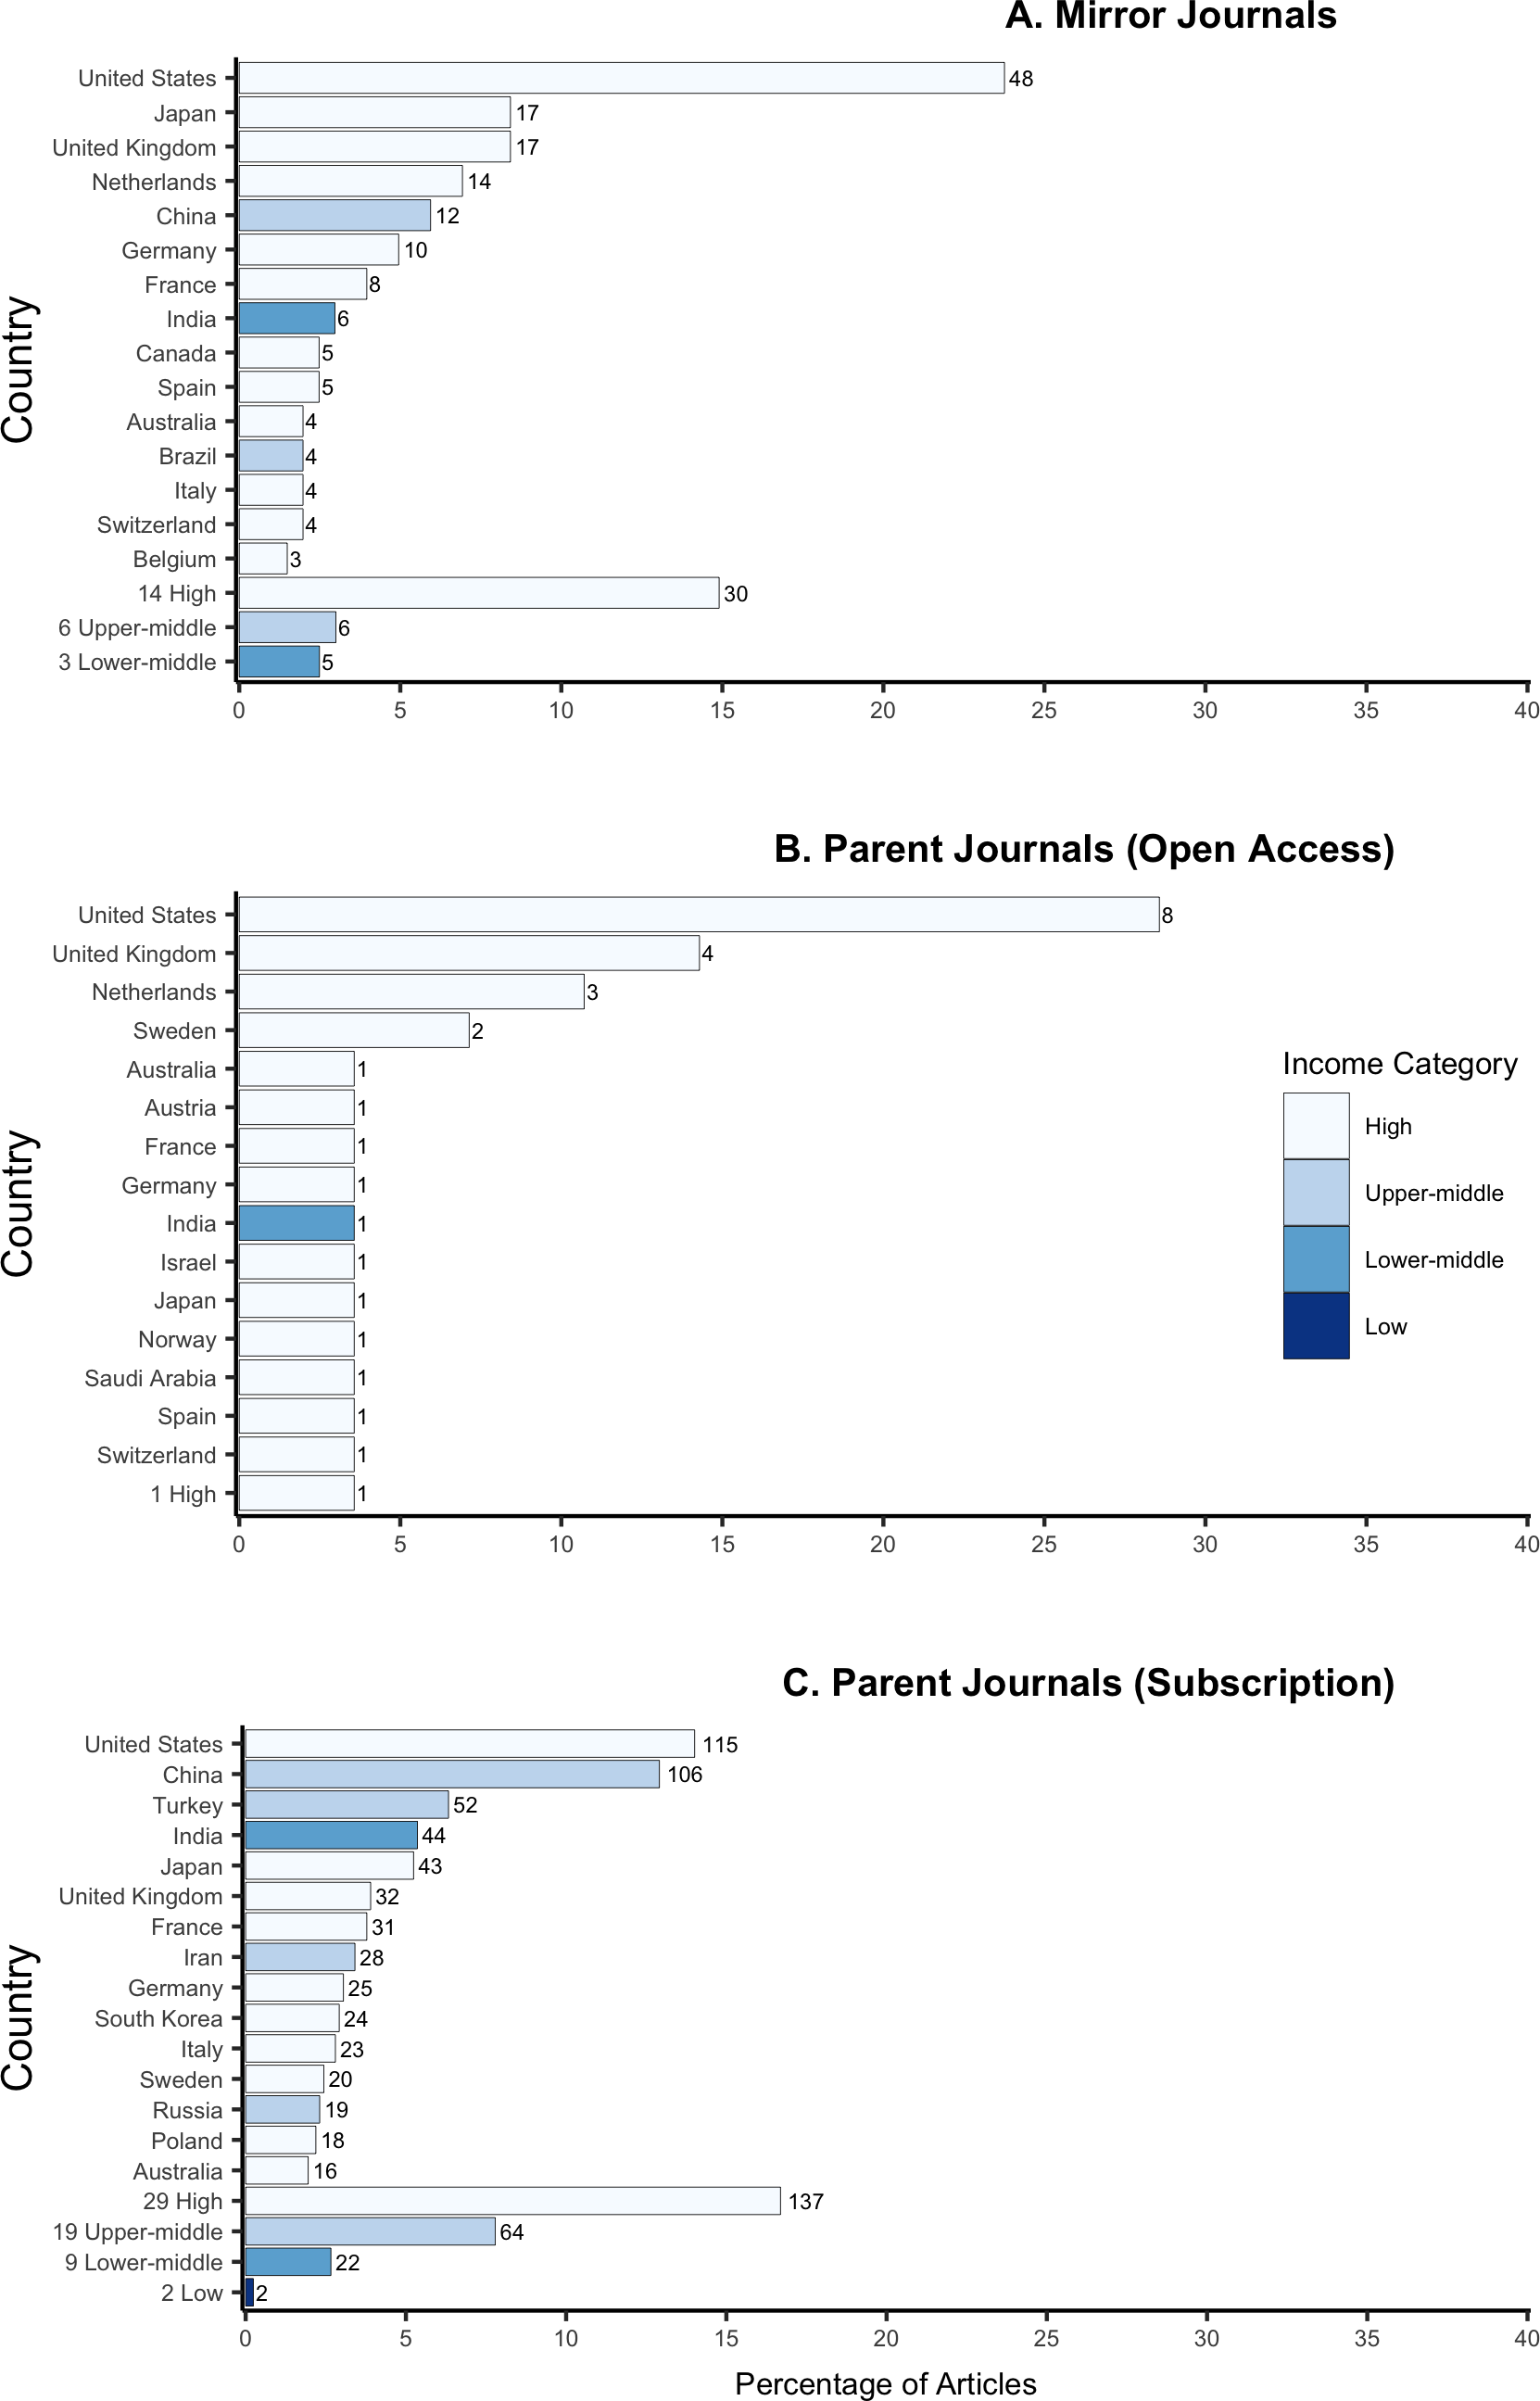
\includegraphics{Smith_etal_APC_ms_files/figure-latex/Fig1-1} 

}

\caption{Percentage of authors of single-author publications in (A) Open Access journals and (B) Paywall journals based in different countries. Numbers adjacent to bars are the number of lead authors based in each country.}\label{fig:Fig1}
\end{figure}

\begin{figure}

{\centering 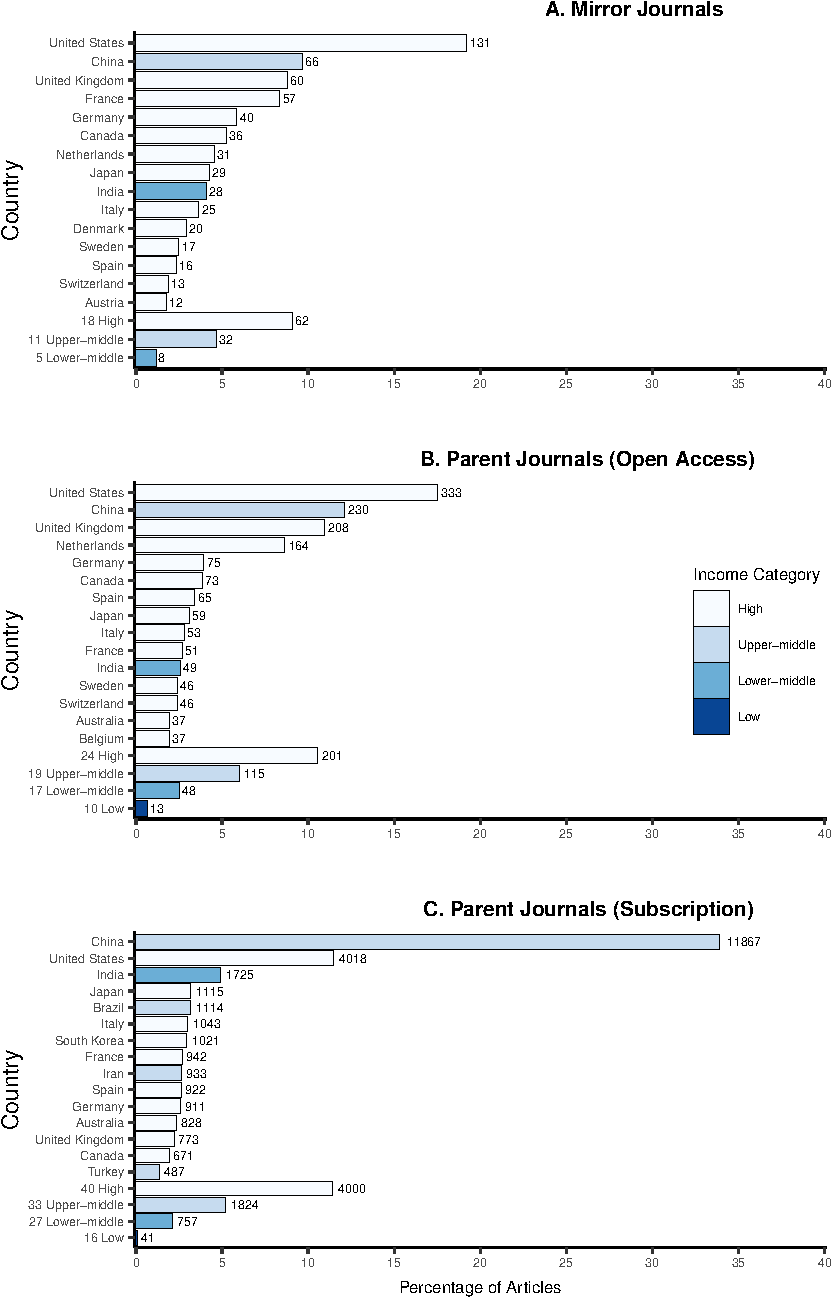
\includegraphics{Smith_etal_APC_ms_files/figure-latex/Fig2-1} 

}

\caption{Percentage of first authors of co-authored publications in (A) Open Access journals and (B) Paywall journals that are based in different countries. Numbers adjacent to bars are the number of lead authors based in each country.}\label{fig:Fig2}
\end{figure}

\begin{figure}

{\centering 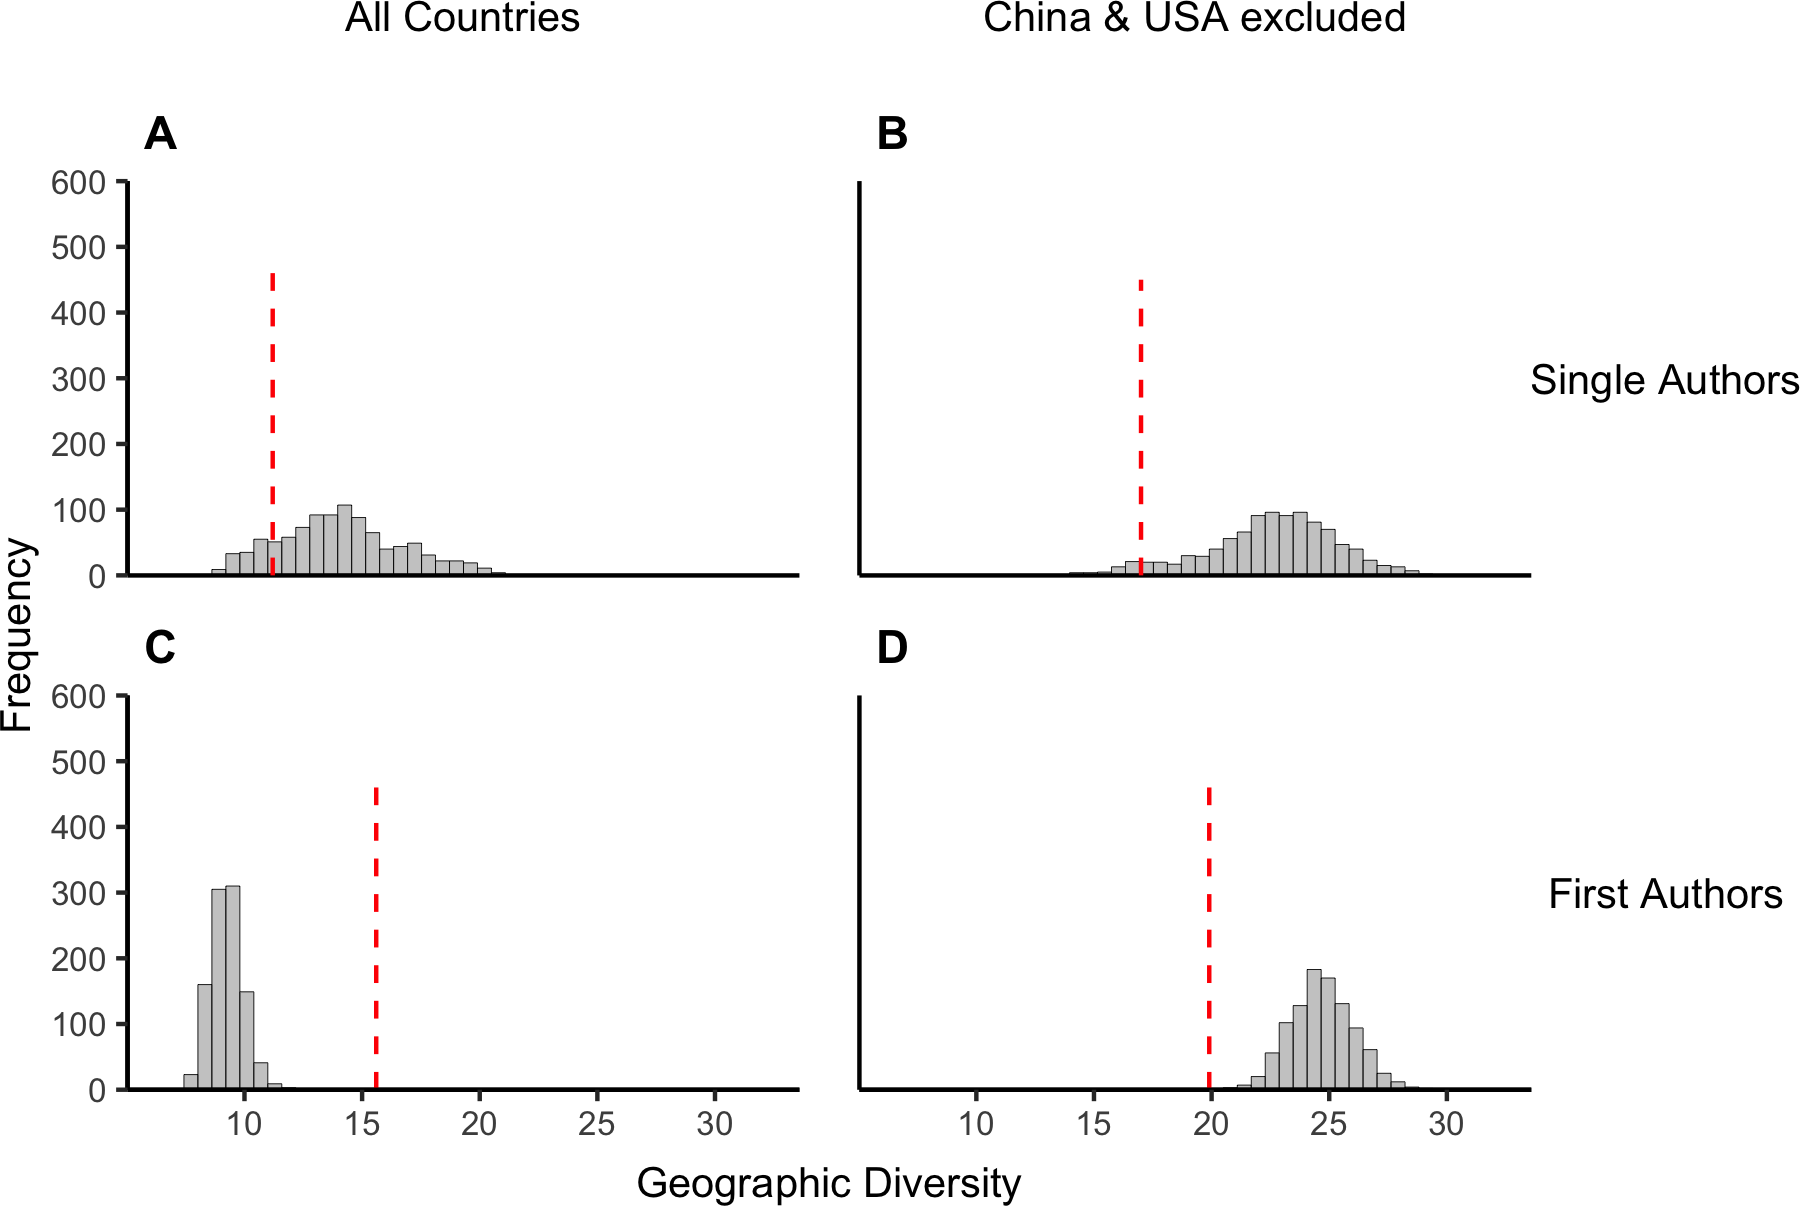
\includegraphics{Smith_etal_APC_ms_files/figure-latex/Fig3-1} 

}

\caption{Author Geographic Richness for N =  984  Open Access articles (red bar) and 1000 identically sized collections of Paywalled articles selected by bootstrapping from a pool of  40330  articles. The black line indicates the mean value for the 1000 bootstrap collections.}\label{fig:Fig3}
\end{figure}

\begin{figure}

{\centering 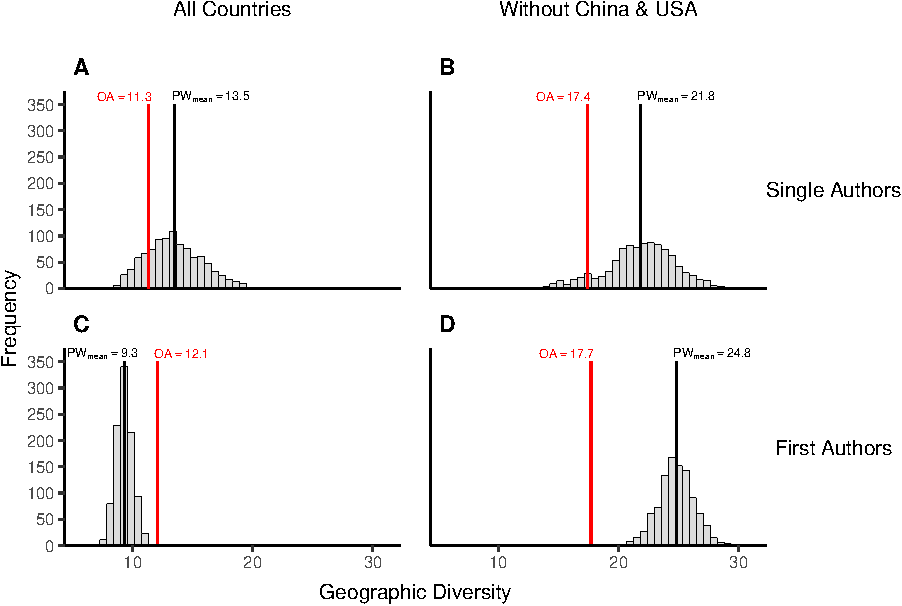
\includegraphics{Smith_etal_APC_ms_files/figure-latex/Fig4-1} 

}

\caption{Author Geographic Diversity ($D_2$) for N =  984  Open Access articles (red bar) and 1000 identically sized collections of Paywalled articles selected by bootstrapping from a pool of  40330  articles.  The black line indicates the mean value for the 1000 bootstrap collections.}\label{fig:Fig4}
\end{figure}

\begin{figure}

{\centering 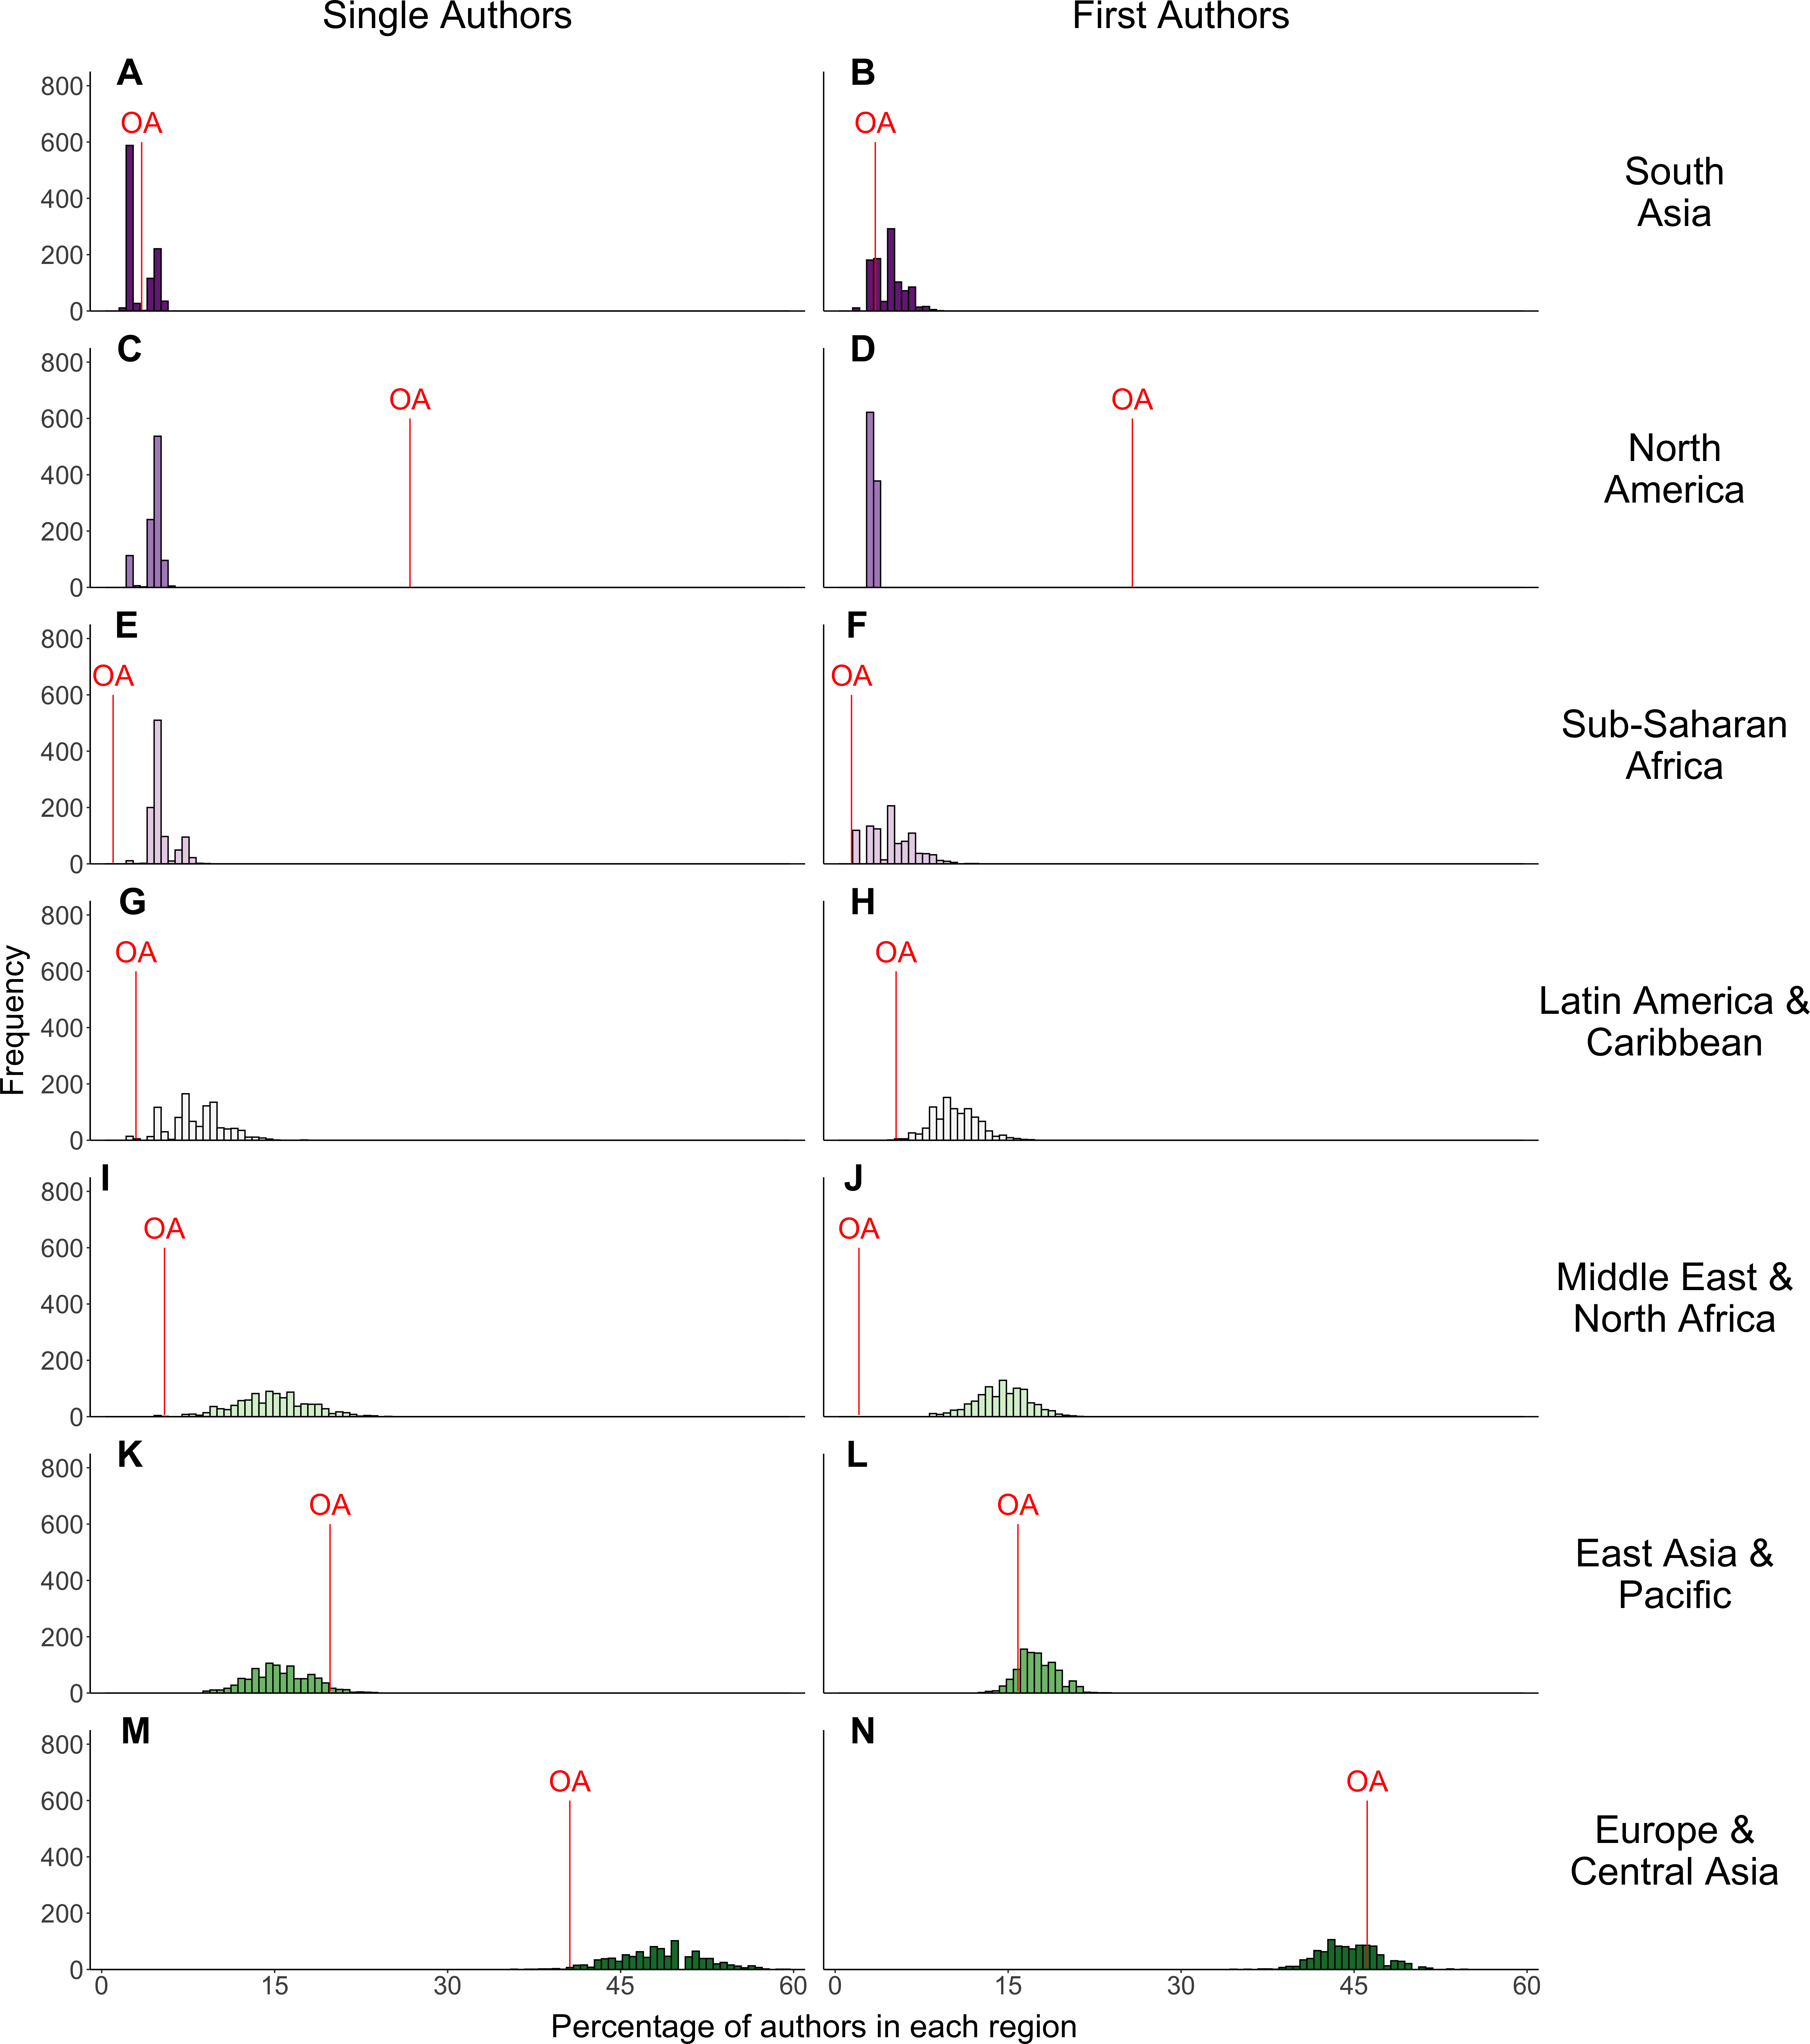
\includegraphics{Smith_etal_APC_ms_files/figure-latex/Fig5-1} 

}

\caption{Percentage of first authors of (A) co-authored and (B) sole-authored open access articles (red bars) and 1000 bootstrapped collections of paywalled articles that are based in different global regions.}\label{fig:Fig5}
\end{figure}

\begin{figure}

{\centering 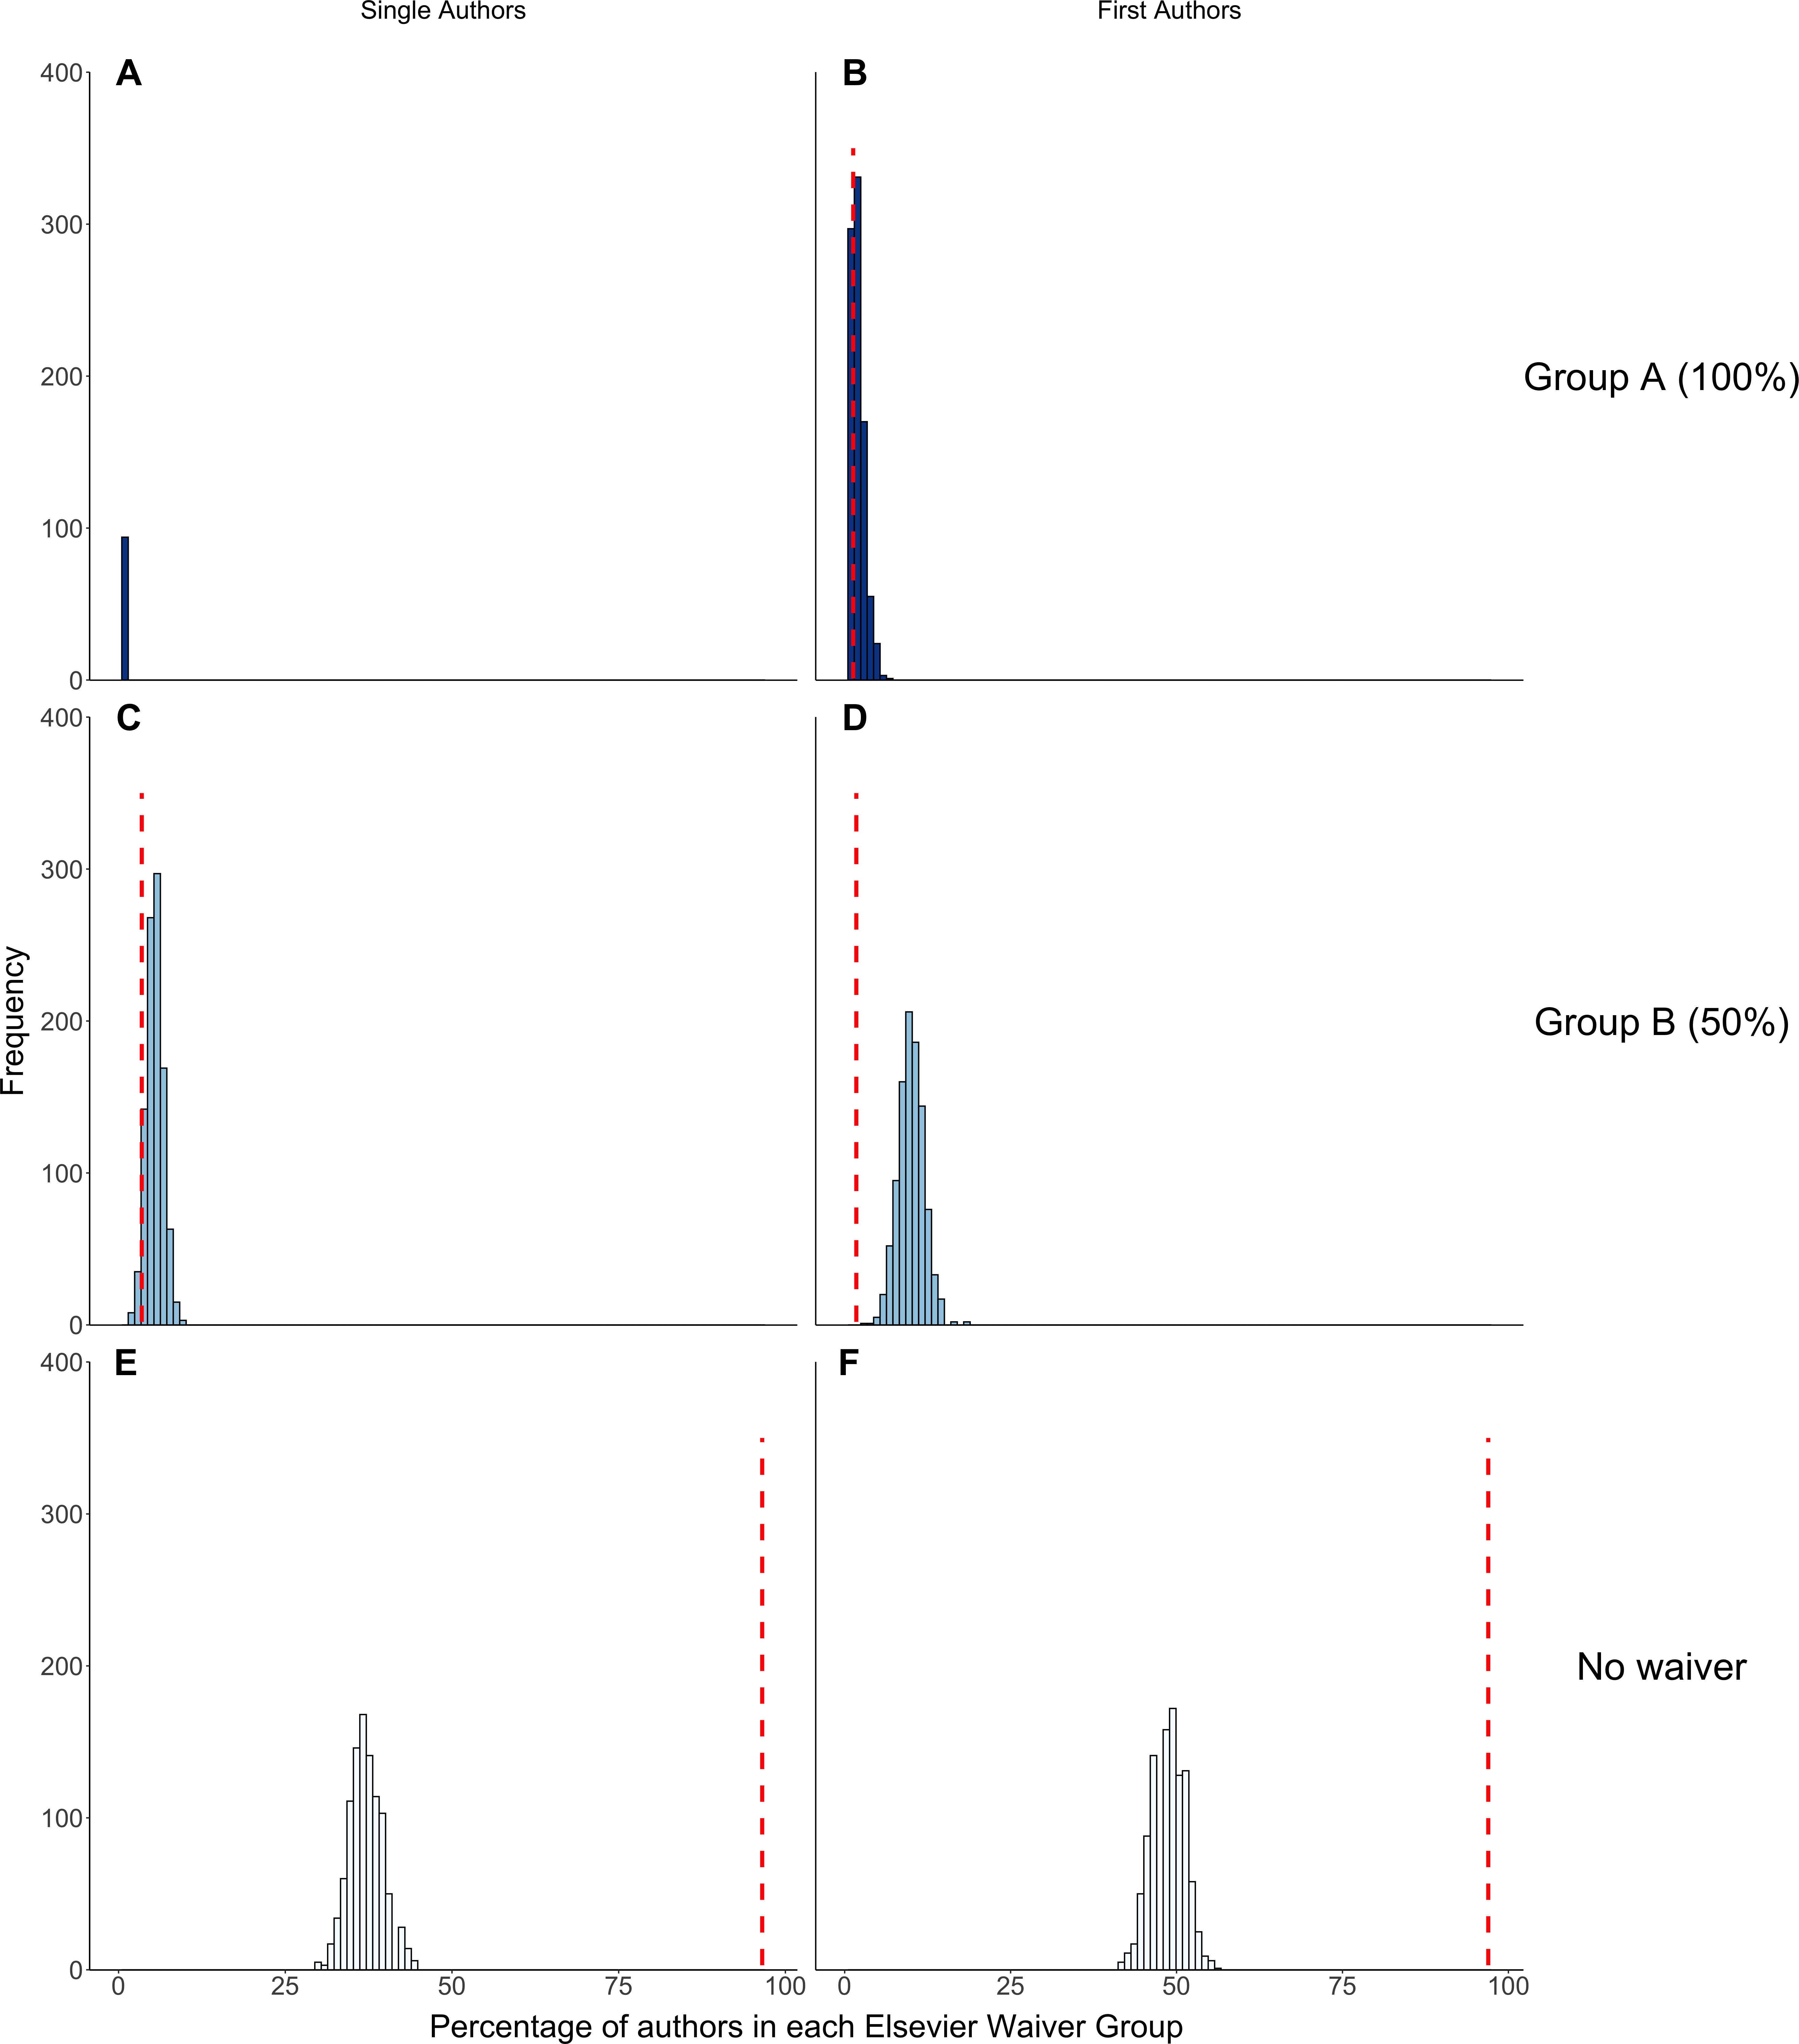
\includegraphics{Smith_etal_APC_ms_files/figure-latex/Fig6-1} 

}

\caption{Percentage of first authors of (A) co-authored and (B) sole-authored open access articles (red bars) and 1000 bootstrapped collections of paywalled articles that are based in different global regions.}\label{fig:Fig6}
\end{figure}

\begin{table}

\caption{\label{tab:Table1}Elsevier subscription journals included in this study, the number of articles published in each one that were included in our study, the number of articles published in each Open Access mirror during the same time period, and the article processing charge (APC) charged by each OA mirror journal. With two exceptions, the titles of paywall and mirror journals are identical except for the 'X' at the end of mirror versions (e.g., Research Policy X, Optical Materials X).}
\resizebox{\linewidth}{!}{
\fontsize{12}{14}\selectfont
\begin{tabular}[t]{lccc}
\toprule
Journal & Articles (PW) & Articles (OA mirror) & APC (US\$)\\
\midrule
Water Research & 2444 & 41 & 3750\\
International Journal of Pharmaceutics & 1412 & 38 & 3700\\
Biosensors and Bioelectronics & 1280 & 9 & 3500\\
Chemical Engineering Science & 1194 & 45 & 3500\\
Respiratory Medicine & 315 & 14 & 3500\\
Resources Conservation and Recycling & 736 & 24 & 3500\\
Cytokine & 514 & 7 & 3400\\
Gene & 1263 & 21 & 3400\\
Sleep Medicine & 456 & 8 & 3360\\
Toxicon & 318 & 26 & 3300\\
Contraception & 219 & 21 & 3200\\
Journal of Hydrology & 1609 & 37 & 3200\\
Veterinary Parasitology & 238 & 21 & 3200\\
Energy Conversion and Management & 1931 & 17 & 3100\\
Chemical Physics Letters & 1315 & 23 & 3050\\
Journal of Dentistry & 233 & 5 & 3000\\
Journal of Biotechnology & 349 & 10 & 2820\\
Food Chemistry & 3670 & 53 & 2800\\
Journal of Computational Physics & 1130 & 35 & 2800\\
Journal of Structural Biology & 220 & 17 & 2750\\
Ecological Engineering & 494 & 13 & 2600\\
Journal of Asian Earth Sciences & 683 & 10 & 2600\\
World Neurosurgery & 3685 & 43 & 2600\\
European Journal of Obstetrics \& Gynecology and Reproductive Biology & 576 & 84 & 2500\\
Vaccine & 1639 & 42 & 2450\\
Research Policy & 264 & 2 & 2400\\
Journal of Biomedical Informatics & 253 & 15 & 2350\\
Atherosclerosis & 404 & 5 & 2308\\
Chaos Solitons and Fractals & 792 & 15 & 2200\\
Expert Systems With Applications & 1211 & 10 & 2200\\
Journal of Non-Crystalline Solids & 848 & 33 & 2200\\
Nutrition & 480 & 2 & 2050\\
Microelectronic Engineering$^{2}$ & 581 & 39 & 2020\\
Materials Letters & 2927 & 30 & 2000\\
Analytica Chimica Acta & 1382 & 19 & 1850\\
Optical Materials & 1184 & 34 & 1500\\
Atmospheric Environment & 1177 & 67 & 1400\\
Biochimie$^{1}$ & 904 & 49 & 1318\\
Total: & 40330 & 984 & \\
\bottomrule
\multicolumn{4}{l}{\textsuperscript{1} OA Mirror title: Biochimie Open}\\
\multicolumn{4}{l}{\textsuperscript{2} OA Mirror title: Micro and Nano Engineering}\\
\end{tabular}}
\end{table}

\begin{table}

\caption{\label{tab:Table2}Geographic Richness and Geographic Diversity of lead authors of papers published in Open Access (OA) and Paywalled (PW) journals. The value for PW is the mean of 1000 bootstrap-generated article collections identical in size to the OA collection. Single: authors of single-authored papers; First: first authors of co-authored papers.}
\centering
\resizebox{\linewidth}{!}{
\fontsize{12}{14}\selectfont
\begin{tabular}[t]{cccccccc}
\toprule
\multicolumn{2}{c}{ } & \multicolumn{3}{c}{All Countries} & \multicolumn{3}{c}{Without China \& USA} \\
\cmidrule(l{3pt}r{3pt}){3-5} \cmidrule(l{3pt}r{3pt}){6-8}
Metric & Author & OA & PW (mean±SD) & $\hat{P}$ & OA & PW (mean±SD) & $\hat{P}$\\
\midrule
Richness & Single & 38.0 & 41.8±2.9 & 0.880 & 36.0 & 39.4±2.8 & 0.853\\
 & First & 60.0 & 60.7±3.3 & 0.528 & 58.0 & 61.8±3.2 & 0.841\\
Diversity & Single & 11.3 & 13.5±2.3 & 0.808 & 17.4 & 21.8 ± 2.9 & 0.915\\
 & First & 12.1 & 9.3±0.7 & 0.001 & 17.7 & 24.8 ± 1.5 & 1.000\\
\bottomrule
\end{tabular}}
\end{table}

\begin{table}

\caption{\label{tab:Table3}Monthly stipends for graduate students in select countries. The value of the stipend in US currency is based on the exchange rate in July 2020.}
\centering
\resizebox{\linewidth}{!}{
\fontsize{12}{14}\selectfont
\begin{tabu} to \linewidth {>{\centering}X>{\centering}X>{\centering}X>{\centering}X}
\toprule
Country & Degree & Agency & Stipend (US\$)\\
\midrule
Brazil & Masters & CNPq$^[1]$ & 282\\
 & Doctorate &  & 413\\
Mexico & Masters & CONACYT$^[2]$ & 493\\
 & Doctorate &  & 711\\
India & Doctorate & SERB$^[3]$ & 737\\
India & Doctorate & RISTEKDIKTI$^[4]$ & 965\\
South Africa & Masters & NRF$^[5]$ & 574\\
 & Doctorate &  & 588\\
\bottomrule
\multicolumn{4}{l}{\textsuperscript{1} http://cnpq.br/apresentacao13/}\\
\multicolumn{4}{l}{\textsuperscript{2} https://www.conacyt.gob.mx/index.php/becas-y-posgrados/becas-nacionales}\\
\multicolumn{4}{l}{\textsuperscript{3} http://www.serb.gov.in/pmfdr.php}\\
\multicolumn{4}{l}{\textsuperscript{4} http://www.serb.gov.in/pmfdr.php}\\
\multicolumn{4}{l}{\textsuperscript{5} https://www.nrf.ac.za}\\
\end{tabu}}
\end{table}

\begin{table}

\caption{\label{tab:Table4}Percentage of Open Access articles with authors based in different World Bank Regions. The value for paywalled journals (PW) is the mean percentage of 1000 bootstrap-generated article collections identical in size to the Open Access (OA) collection. Single: authors of single-authored papers; First: first authors of co-authored papers; Significant differences between the open access collection and bootstrapped paywall collections are indicated with an asterisk.}
\centering
\resizebox{\linewidth}{!}{
\fontsize{12}{14}\selectfont
\begin{tabular}[t]{cccccc}
\toprule
Author & Countries & Region & PW & OA & \$\textbackslash{}hat\{P\}\$\\
\midrule
Single & All Countries & East Asia \& Pacific & 15.49 & 19.80 & 0.946\\
 &  & Europe \& Central Asia & 48.42 & 40.59 & 0.016*\\
 &  & Latin America \& Caribbean & 8.28 & 2.97 & 0.018*\\
 &  & Middle East \& North Africa & 14.81 & 5.45 & 0.005*\\
 &  & North America & 4.52 & 26.73 & 1*\\
 &  & South Asia & 3.30 & 3.47 & 0.626\\
 &  & Sub-Saharan Africa & 5.20 & 0.99 & 0*\\
First & All Countries & East Asia \& Pacific & 17.60 & 15.85 & 0.138\\
 &  & Europe \& Central Asia & 44.65 & 46.13 & 0.74\\
 &  & Latin America \& Caribbean & 10.45 & 5.28 & 0.002*\\
 &  & Middle East \& North Africa & 14.49 & 2.06 & 0*\\
 &  & North America & 3.31 & 25.77 & 1*\\
 &  & South Asia & 4.66 & 3.48 & 0.288\\
 &  & Sub-Saharan Africa & 4.88 & 1.42 & 0*\\
\bottomrule
\end{tabular}}
\end{table}

\begin{table}

\caption{\label{tab:Table5}Percentage of Open Access articles with authors based in different World Bank Lending Groups. The value for paywalled journals (PW) is the mean percentage of the 1000 bootstrap-generated article collections identical in size to the Open Access (OA) collection. Single: authors of single-authored papers. First: first authors of co-authored papers. Significant differences between the open access collection and bootstrapped paywall collections are indicated with an asterisk.}
\centering
\resizebox{\linewidth}{!}{
\fontsize{10}{12}\selectfont
\begin{tabular}[t]{cccccc}
\toprule
Author & Countries & Lending Group & PW & OA & $\hat{P}$\\
\midrule
Single & All Countries & High & 58.96 & 83.66 & 1*\\
 &  & Lower middle & 10.35 & 5.45 & 0.045*\\
 &  & Upper middle & 30.49 & 10.89 & 0*\\
First & All Countries & High & 56.89 & 81.06 & 1*\\
 &  & Lower middle & 13.71 & 4.64 & 0*\\
 &  & Upper middle & 27.75 & 14.30 & 0*\\
\bottomrule
\end{tabular}}
\end{table}


\clearpage
\makeatletter
\efloat@restorefloats
\makeatother


\begin{appendix}
\section{}
\begin{figure}

{\centering 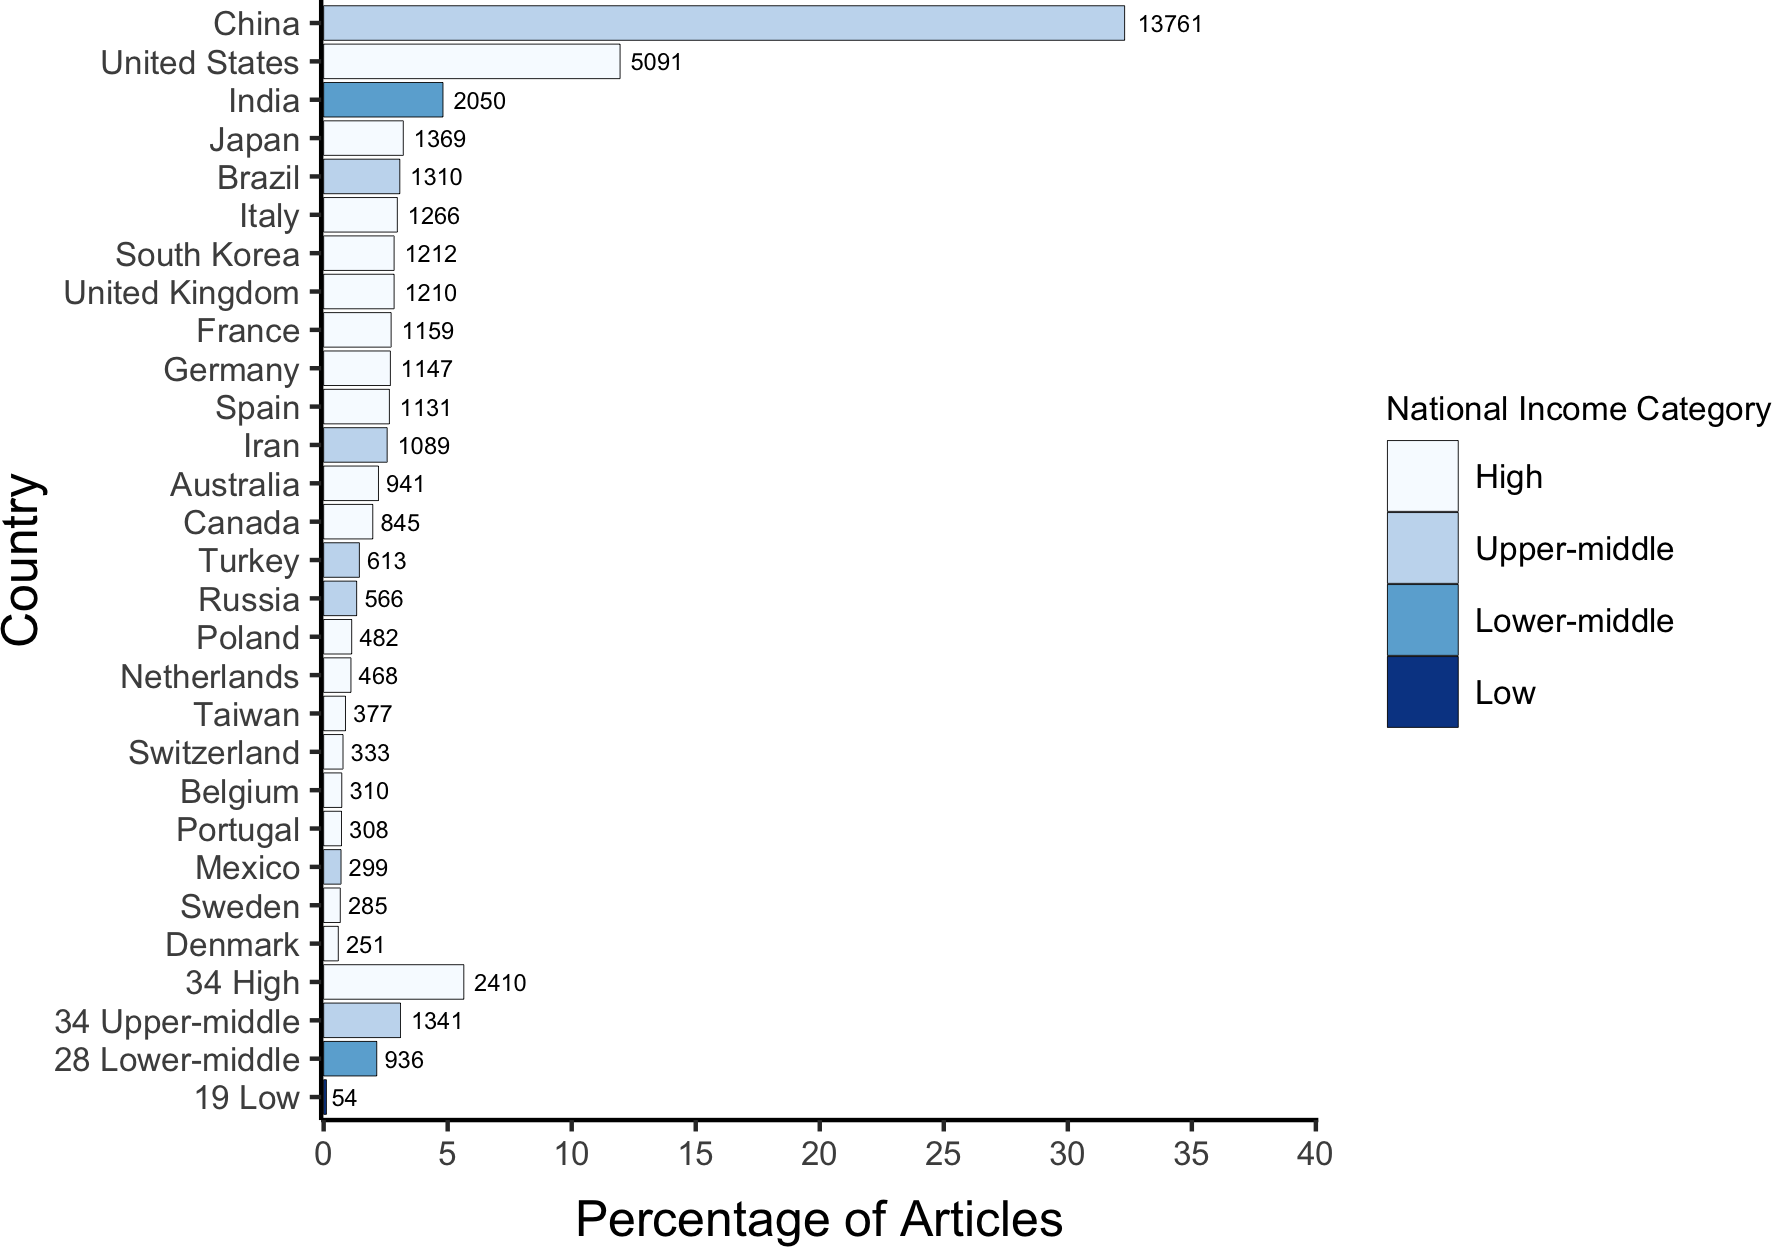
\includegraphics{Smith_etal_APC_ms_files/figure-latex/FigA1-1} 

}

\caption{Percentage of lead authors based in different countries. Includes both paywalled and open access journals. Lead authors includes the authors of sole-authored papers and first authors of co-authored papers. Numbers adjacent to bars are the number of lead authors based in each country.}\label{fig:FigA1}
\end{figure}

\begin{figure}

{\centering 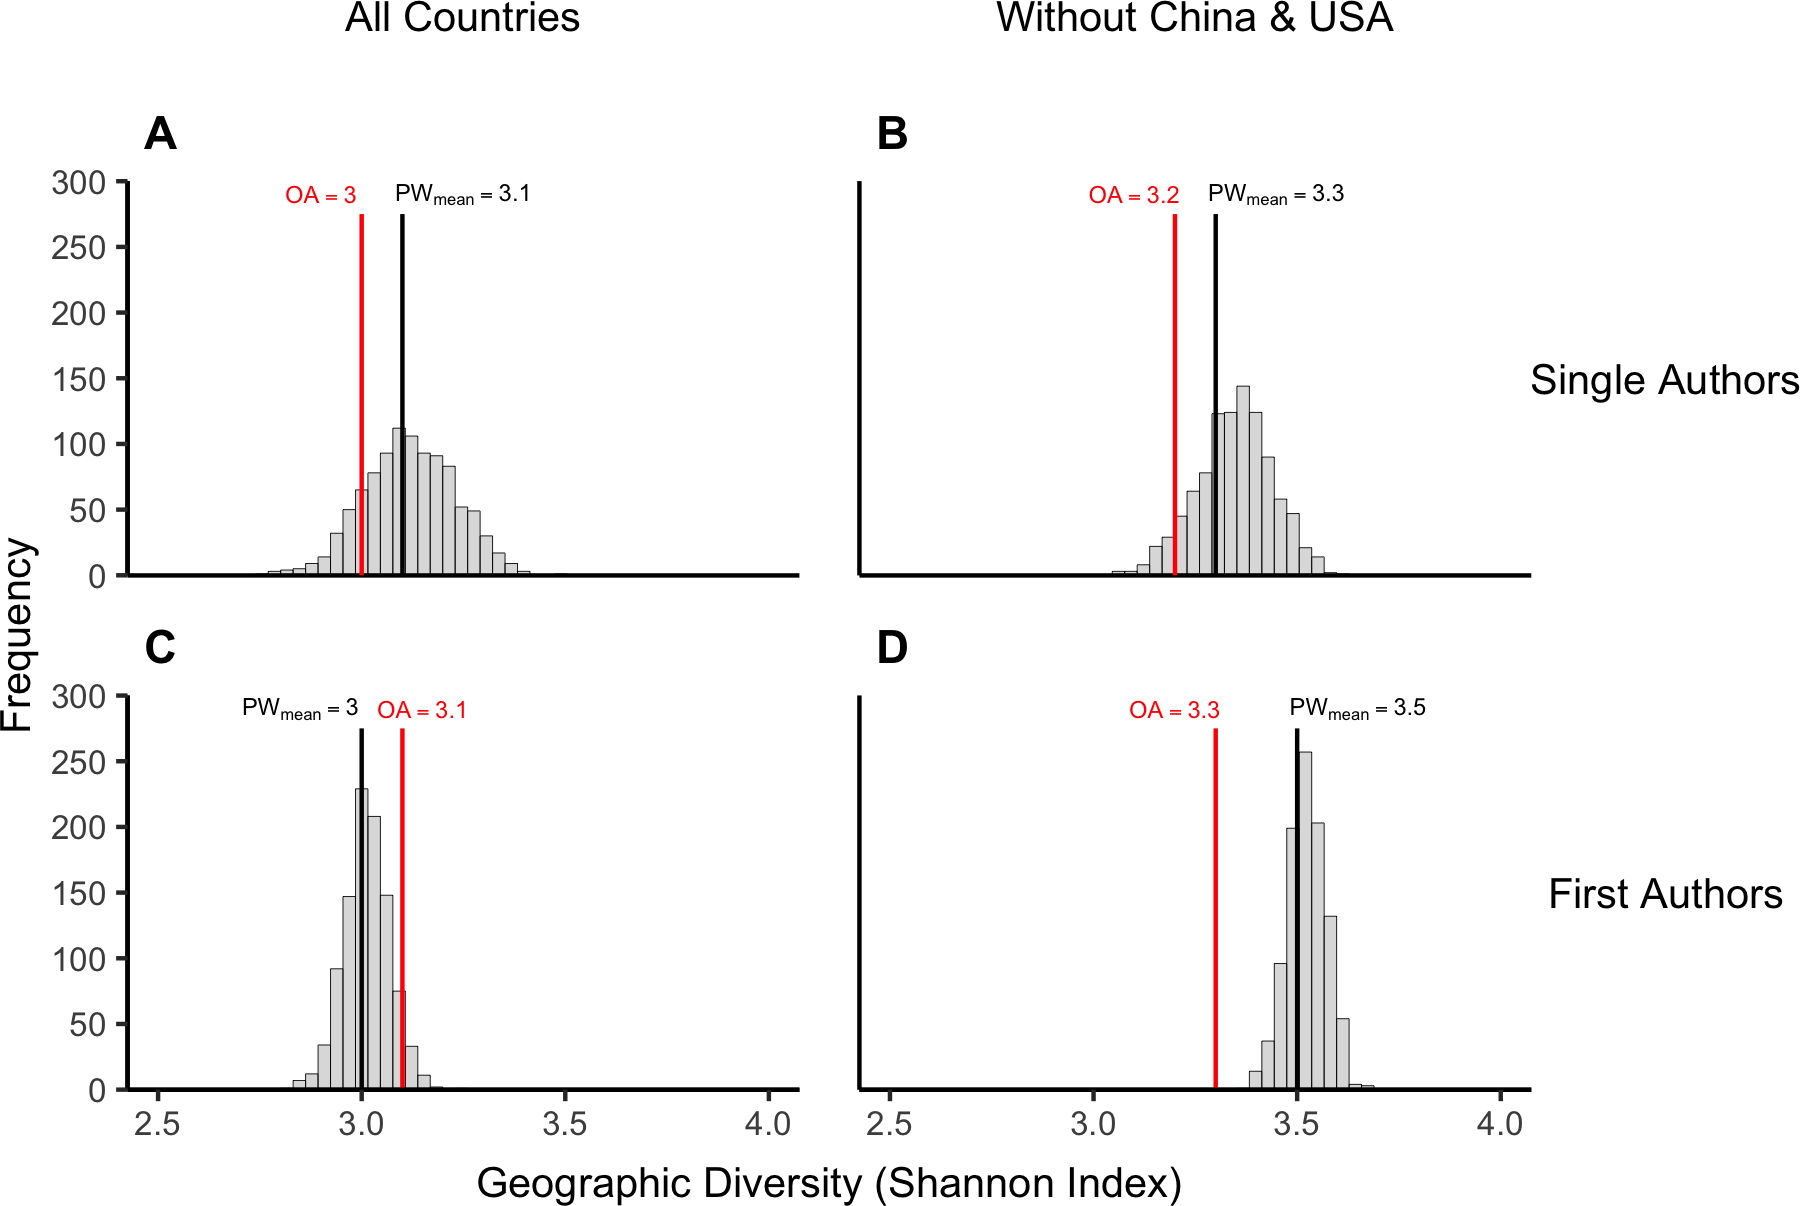
\includegraphics{Smith_etal_APC_ms_files/figure-latex/FigA2-1} 

}

\caption{Author Geographic Diversity (Shannon Index) for N =  984  Open Access articles (red bar) and 1000 identically sized collections of Paywalled articles selected by bootstrapping from a pool of  40330  articles. The black line indicates the mean value for the 1000 bootstrap collections.}\label{fig:FigA2}
\end{figure}

\begin{figure}

{\centering 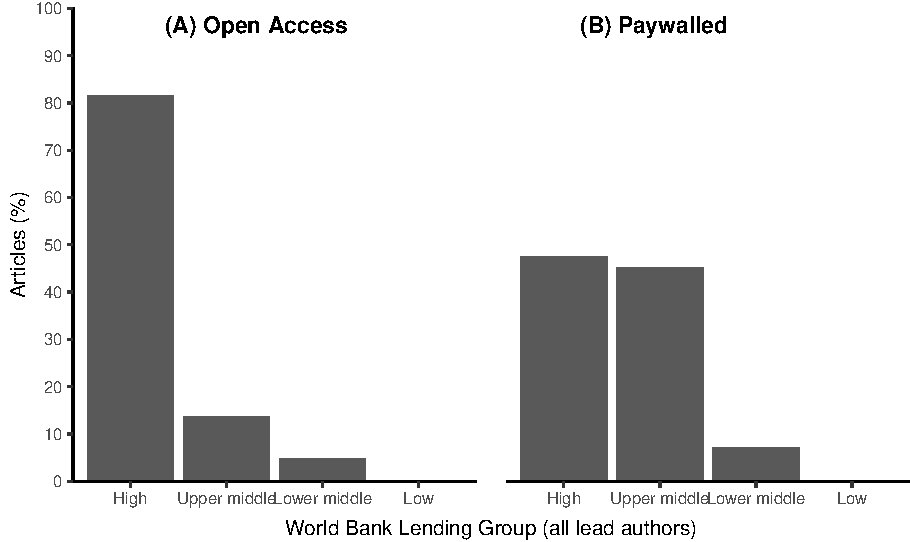
\includegraphics{Smith_etal_APC_ms_files/figure-latex/FigA3-1} 

}

\caption{Proportion of (A) the N =  984  lead authors of Open Access articles and N =   40330  authors of paywalled articles that are based in different World Bank Lending Groups.}\label{fig:FigA3}
\end{figure}

\newpage
\blandscape
\begin{table}

\caption{\label{tab:AppTable}Countries eligible for APC waivers through Elsevier's 'Research4Life' program by World Bank Global Region and Income Group.}
\resizebox{\linewidth}{!}{
\fontsize{12}{14}\selectfont
\begin{tabular}[t]{ccccc}
\toprule
Region & Income Group & A - 100\% & B - 50\% & no waiver\\
\midrule
South Asia & Low income & Afghanistan, Nepal & - & -\\
& Middle income & Bangladesh, Bhutan & Maldives, Pakistan, Sri Lanka & India\\
\cline{1-5}
Sub-Saharan Africa & Low income & Benin, Burkina Faso, Burundi & - & -\\
&  & Central African Republic, Chad, Dem. Repub. Congo, Eritrea & - & -\\
&  & Ethiopia, Gambia, Guinea, Guinea-Bissau & - & -\\
&  & Liberia, Madagascar, Malawi, Mali & - & -\\
&  & Mozambique, Niger, Rwanda, Sierra Leone & - & -\\
&  & Somalia, South Sudan, Tanzania, Togo & - & -\\
&  & Uganda & - & -\\
& Middle income & Angola, Cabo Verde, Cameroon & Botswana, Gabon, Mauritius & South Africa\\
&  & Comoros, Congo, Equatorial Guinea, Eswatini & Namibia, Nigeria & -\\
&  & Ghana, Ivory Coast, Kenya, Lesotho & - & -\\
&  & Mauritania, Sao Tome \& Principe, Senegal, Sudan & - & -\\
&  & Zambia, Zimbabwe & - & -\\
& High income & - & Seychelles & -\\
\cline{1-5}
Latin America \& Caribbean & Low income & Haiti & - & -\\
& Middle income & Belize, Nicaragua & Bolivia, Colombia, Cuba & Argentina, Brazil, Costa Rica\\
&  & - & Dominica, Ecuador, El Salvador, Grenada & Dominican Republic, Mexico\\
&  & - & Guatemala, Guyana, Honduras, Jamaica & -\\
&  & - & Paraguay, Peru, Saint Lucia, Saint Vincent \& the Grenadines & -\\
&  & - & Suriname, Venezuela & -\\
& High income & - & Antigua \& Barbuda, Saint Kitts \& Nevis & Aruba, Bahamas, Barbados\\
&  & - & - & British Virgin Islands, Cayman Islands, Chile, Curaçao\\
&  & - & - & Panama, Puerto Rico, Saint Martin (FRA), Sint Maarten\\
&  & - & - & Trinidad \& Tobago, Turks \& Caicos Islands, U.S. Virgin Islands, Uruguay\\
\cline{1-5}
Middle East \& North Africa & Low income & Syrian Arab Republic, Yemen & - & -\\
& Middle income & Djibouti & Algeria, Egypt, Iraq & Iran, Lebanon\\
&  & - & Jordan, Libya, Morocco, Tunisia & -\\
&  & - & West Bank \& Gaza Strip & -\\
& High income & - & - & Bahrain, Israel, Kuwait\\
&  & - & - & Malta, Oman, Qatar, Saudi Arabia\\
&  & - & - & United Arab Emirates\\
\cline{1-5}
E. Asia \& Pacific & Low income & Democratic People’s Republic  Korea & - & -\\
& Middle income & Cambodia, Fed. States  Micronesia, Kiribati & Fiji, Mongolia, Nauru & American Samoa, China, Indonesia\\
&  & Laos, Marshall Islands, Myanmar, Papua New Guinea & Vietnam & Malaysia, Philippines, Thailand\\
&  & Samoa, Solomon Islands, Timor-Leste, Tonga & - & -\\
&  & Tuvalu, Vanuatu & - & -\\
& High income & - & Palau & Australia, Brunei, French Polynesia\\
&  & - & - & Guam, Hong Kong, Japan, Macao\\
&  & - & - & N. Mariana Islands, New Caledonia, New Zealand, Singapore\\
&  & - & - & South Korea, Taiwan\\
&  & Tokelau & Cook Islands, Niue & -\\
\cline{1-5}
Europe \& Central Asia & Low income & Tajikistan & - & -\\
& Middle income & Kyrgyzstan, Republic  Moldova & Albania, Armenia, Azerbaijan & Bulgaria, Kazakhstan, Romania\\
&  & - & Belarus, Bosnia \& Herzegovina, Georgia, Kosovo & Russia, Turkey, Turkmenistan\\
&  & - & Montenegro, North Macedonia, Serbia, Ukraine & -\\
&  & - & Uzbekistan & -\\
& High income & - & - & Andorra, Austria, Belgium\\
&  & - & - & Croatia, Cyprus, Czechia, Denmark\\
&  & - & - & Estonia, Faroe Islands, Finland, France\\
&  & - & - & Germany, Gibraltar, Greece, Greenland\\
&  & - & - & Hungary, Iceland, Ireland, Isle  Man\\
&  & - & - & Italy, Latvia, Liechtenstein, Lithuania\\
&  & - & - & -\\
&  & - & Saint Helena & -\\
\cline{1-5}
North America & High income & - & - & Bermuda, Canada, United States\\
\bottomrule
\end{tabular}}
\end{table}
\elandscape
\end{appendix}

\end{document}
